\chapter{Chiral Subtleties in Charged Lepton Flavor Physics}
\label{lfv}

%https://arxiv.org/pdf/1607.01022


%https://journals.aps.org/prl/pdf/10.1103/PhysRevLett.120.221804\\
%https://arxiv.org/pdf/1709.00294\\
%https://arxiv.org/pdf/1610.06587\\
%https://arxiv.org/pdf/1303.4097

%Couples chirally: \\
%https://arxiv.org/pdf/1610.08060

%tau:\\
%https://arxiv.org/pdf/2406.15286v2

%Charged Lepton Flavor Violation:
%https://arxiv.org/pdf/2209.00142
%sec. 6.4
% Future limits: https://arxiv.org/pdf/1711.08430

%https://arxiv.org/pdf/0909.5148
\section{Introduction}
As we have discussed in the Introduction and Chapters \ref{fv_qft}, lepton flavor violation (LFV) is a hallmark of many extensions to the SM, and is hence a promising avenue to search for new physics. This chapter will explore spin-zero particles with generically flavor-violating and CP-violating interactions to the SM charged leptons. For simplicity, we assume that these particles are {\it leptophilic}, so they couple only to the lepton sector of the SM. It is not too difficult to provide charge assignments in the UV that forbid direct interaction with quarks. As examples, we refer to lepton-specific 2HDM models \cite{Cao:2009as}, gauged $U(1)_{L_i-L_j}$ extensions to the SM \cite{Foot:1990mn,He:1990pn,He:1991qd,Heeck:2011wj}, and the composite dark matter model in Ref.~\cite{Davoudiasl:2017zws} which is reviewed in  Section \ref{sec:composite_ALP}. That said, most of our results are independent of this choice, with the exception being the induced photonic coupling one finds when treating an LFV ALP interaction with the (pseudo)-scalar current (which would have a contribution from quarks in more generic models).

We have already seen in Chapter \ref{fv_qft} that chirally coupled particles can appear naturally as low-energy modes of some extensions to the SM. We have also encountered two scenarios where ALPs appear in the low energy theory with purely chiral interactions with the leptons. The appearance of particles with chiral interactions is not too surprising given that the Standard-Model fermion fields themselves are Weyl fermions prior to EWSB, with the Dirac structure only emerging after imposing unitary gauge and diagonalizing the SM quadratic terms. While mixing sometimes spoils the pure chiral nature of the interactions (as is the case when the $W_3$ mixes with the $B$ to make the $Z$ boson), this is not guaranteed to happen (as is the case with the $(W_1\pm iW_2 )/\sqrt{2}= W_{\pm}$ bosons), so we believe the chiral scenario should be examined more closely.

In this chapter, we will consider the leading constraints on the LFV couplings of scalars and ALPs, exploring the role of PV and CPV in the process. In Section \ref{sec:lfv_int}, we will examine how a chiral interaction (and more exotic PV and CPV interactions) may arise from interactions involving the SM gauge fields prior to EWSB. In Section \ref{sec:lfv_decays}, we will consider the limits one can obtain from LFV decay modes of the $\mu$ and $\tau$ leptons, comparing ``pure'' (parity-conserving) interactions to chiral interactions for both scalars and ALPs. Finally, in Section \ref{sec:edm_mdm}, we consider the contribution of LFV scalars and ALPs to the lepton electric and magnetic dipole moments. The electric dipole moments receive no contribution from pure or chiral interactions because these interactions preserve CP, so in this case we consider limits on the degree of CP violation in the coupling. For the magnetic dipole moments, we explore LFV scalar and ALP explanations for the electron and muon $g-2$ anomalies, and also place limits on the couplings in the event that these anomalies are resolved. Throughout this chapter, we will refer to the boson as the $\varphi$ and its mass as $m_\varphi$ unless we are specializing to an ALP-specific scenario, for which we will refer to it as the $a$ with mass $m_a$.

\section{LFV Interaction}\label{sec:lfv_int}

\subsection{UV Considerations}\label{sec:lfv_uv}
In this section, we will review some scenarios in which LFV scalars can arise naturally from some UV model. We will focus on two concrete examples: an additional Higgs doublet, and an ALP coupled to the lepton sector.
\begin{center}
    {\it 1. Higgs Doublet}
\end{center}
We begin by examining the interaction between a second Higgs doublet $\Phi$ and the leptons. For simplicity, we will assume that the SM Higgs-lepton interaction is already diagonalized, so that we are operating with the SM lepton eigenstates.\footnote{If the $\Phi$ acquires a VEV, these are not the true eigenstates of the low-energy theory.}Then, the $\Phi$-lepton interaction is given by
\begin{align}
     {\cal L}_{\rm int} = \sum_{i,j}\left[y_{ij}\bar{L}_i \Phi \ell_{jR} + y_{ji}^*\bar{\ell}_{iR}\Phi^\dagger L_j\right]
\end{align}
In the following, we will only focus on interactions with the charged leptons, so we will isolate the charge-neutral component of the Higgs doublet, $\Phi^0$:
\begin{align}
{\cal L}_{\rm int} &= \sum_{i,j}\left[y_{ij}\Phi^0\bar{\ell}_i P_R \ell_j + y_{ji}^*\Phi^{0\dagger}\bar{\ell}_i P_L\ell_j \right] + \cdots
\end{align}
Due to the nature of the $SU(2)$ symmetry, the $\Phi^0$ coupling is chiral: a $\Phi^0$ can only decay to an $\ell_L^- \ell_R^+$, not an $\ell_R^-\ell_L^+$. Since $\Phi^0$ is a complex scalar, it can be split into real and imaginary parts, $\Phi^0 \equiv s + ia$. Depending on the potential between the $\Phi$ and other scalars, the $s$ and $a$ may acquire a significant mass splitting after diagonalizing the quadratic interaction, so it is instructive to treat each of them as separate fields and see whether any notion of ``chirality'' persists. Doing so, we find the following interaction term:
\begin{align}
{\cal L}_{\rm int} &= \sum_{i,j}\left\{s\bar{\ell}_i\left[ y_{ij}P_R  + y_{ji}^*P_L\right]\ell_j+ ia\bar{\ell}_i\left[ y_{ij}P_R  - y_{ji}^*P_L\right]\ell_j\right\}
\end{align}
It is worth examining these interactions using the magnitude, angle, and phase formalism described in Section \ref{sec:FV_scalar_CPT}. Then, the magnitude, angles and phases for the scalar $s$ are given by
\begin{align}
    g_{ij}^s &= \sqrt{\frac{|y_{ij}|^2 + |y_{ji}|^2}{2}}\\
    -ie^{i\delta_{ij}^s}\tan{\theta_{ij}^s} &= \frac{y_{ij} - y_{ji}^*}{y_{ij} + y_{ji}^*},
\end{align}
and the magnitudes, angles and phases for the pseudoscalar $a$ are given by
\begin{align}
    g_{ij}^a &= \sqrt{\frac{|y_{ij}|^2 + |y_{ji}|^2}{2}}\\
    -ie^{i\delta_{ij}^a}\tan{\theta_{ij}^a} &= \frac{y_{ij} + y_{ji}^*}{y_{ij} - y_{ji}^*}.
\end{align}
The parameters for the $s$ and $a$ are related: $g_{ij}^a = g_{ij}^s$, $\delta_{ij}^a = - \delta_{ij}^s$, and $\theta_{ij}^a = \pi/2 - \theta_{ij}^s$. Note that the $s$ is a ``pure'' scalar and $a$ a ``pure'' pseudoscalar only  when $y_{ij} = y_{ji}^*$ (i.e., when the Yukawa matrix ${\bf y}$ is Hermitian), but there is no reason to expect this in general. The only reason the SM Higgs Yukawa matrices are Hermitian and diagonal is because we redefined the fields to diagonalize the mass matrix and make it so; any additional Higgs doublet interactions do not have this luxury, and even the SM Higgs interaction in principle does not have this luxury if there are other Higgs doublets which acquire a VEV. Something interesting happens when $y_{ij} \neq 0$ but $y_{ji} = 0$ (which can occur in interactions with explicit flavor symmetries, such as  Froggatt-Nielsen models\footnote{In this case, the Higgs Yukawas have this property {\it prior} to diagonalization of the mass matrix, but one could imagine a similar effect with a second Higgs doublet coupled to the Froggatt-Nielsen scalar.}\cite{Froggatt:1978nt,Greljo:2024evt} and gauged $U(1)_{L_i - L_j}$ models with charged Higgs doublets \cite{Heeck:2011wj}). Then, $\theta_{ij}^{s,a} = -\theta_{ji}^{s, a} = \pi/4$, and $\delta_{ij}^{s,a} = \delta_{ji}^{s,a} =\pm\pi/2$, so the $s$ and $a$ fields are also chiral. More generally, it is easy to convince oneself that the fraction on the right can be any complex number, so the angles and phases can take on any value depending on the complex texture of the Yukawa couplings. Near-chiral interactions may arise if there is only an approximate flavor symmetry for which $|y_{ji}|\ll |y_{ij}|$. One can expect more complicated behavior in the event that the real and imaginary parts are not eigenstates of the low-energy theory, but that is beyond the scope of this discussion. 

One important difference between complex chiral scalars and real chiral scalars is the flavor-diagonal couplings. In particular, one cannot have $y_{ii}^* = 0$ but $y_{ii} \neq 0$, so there can be no ``chiral coupling'' of scalars to the flavor-conserving scalar current. The same is not true for a complex scalar. One might object that a complex scalar is just two real scalars, so how can one have a chiral coupling and not the other? The key is that if the $s$ and $a$ have the same mass, they have the same propagator, so for $i = j$ their contributions to Feynman diagrams can cancel exactly to give the effect of a chiral coupling to the flavor-conserving scalar currents.
\begin{center}
    {\it 2. Leptophilic Axion-Like Particle}
\end{center}
If an ALP comes from some approximate global symmetry in a UV model, it will not couple directly to the SM fermion eigenstates, but the SM gauge fields. In full generality, the ALP will couple with different coefficients to the left-handed lepton doublets and right-handed lepton singlets: 
\begin{align}
    {\cal L}_{\rm int} &= \frac{\partial_\mu a}{\Lambda} \, \sum_{i,j}\left[C^L_{ij}\bar{L}_i\gamma^\mu L_j + C^R_{ij}\, \bar{\ell}_{Ri}\gamma^\mu \ell_{Rj}\right]
\end{align}
To ensure Hermiticity of the Lagrangian, we must have $C_{ij}^L = C_{ji}^{L*}$ and $C_{ij}^R = C_{ji}^{R*}$ because $a$ is real. Of course, it is possible to express this interaction in terms of the lepton eigenstates of the SM. Focusing only on the charged leptons,\footnote{The ALP interaction can be completely rotated away in the neutrino sector provided they are massless.} we have 
\begin{align}
    {\cal L} &= \frac{\partial_\mu a}{\Lambda} \, \sum_{i,j}\bar{\ell}_i\gamma^\mu\left[C_{ij}^LP_L + C_{ij}^R P_R\right]\ell_j\label{eq:ALP_int_from_UV}
\end{align}
In this case, if one of $C_{ij}^R$ or $C_{ij}^L$ is zero, then the ALP has a chiral coupling to the charged leptons. We have encountered this in Chapter \ref{fv_qft} both for the axiflavon with certain Froggatt-Nielsen textures, and for the composite ALP model. Rewriting the left-right projection operators as $P_{R(L)} = \tfrac{1}{2}(1\pm\gamma^5)$, we see that the vector and axial-vector coupling strengths are $A_{ii} = C_{ij}^R - C_{ij}^L$ and $V_{ii} = C_{ij}^R + C_{ij}^L$. We can use the notation from Section \ref{sec:ALP_as_pseudoscalar} to decompose the couplings into magnitudes, angles, and phases:
\begin{align}
    C_{ij} &= \sqrt{\frac{|C_{ij}^L|^2 + |C_{ij}^R|^2}{2}}\\
    e^{i\Delta_{ij}}\tan{\Theta_{ij}} &= \frac{C_{ij}^R + C_{ij}^L}{C_{ij}^R - C_{ij}^L}.
\end{align}
Hermiticity requires $\Delta_{ji} = -\Delta_{ij}$ and $\Theta_{ji} = -\Theta_{ij}$. The ALP couples to the axial-vector current only when $C_{ij}^L = -C_{ij}^R$, which is an arbitrary choice that would only apply to very specific UV models. In the event that $C_{ij}^R = C_{ij}^L$, $\Theta_{ij} = \pi/2$ and the ALP will couple directly to the vector current. This scenario has interesting implications, because the absence of an axial vector current in the interaction effectively removes the on-diagonal interaction. This is easier to see when the ALP interaction is rewritten to be scalar-like; substituting $\Theta_{ii} = 0$ into the effective scalar coupling in Eq.~\ref{eq:ALP_to_scalar} reveals $g_{ii} = \frac{C_{ii}}{\Lambda}\sqrt{m_i^2 + m_i^2 + 2m_i m_i \cos{\pi}} = 0$. As we will see, an ALP with this property would evade many of the existing constraints from LFV lepton decay modes, because most of the diagrams that contribute in these channels involve one on-diagonal coupling and one off-diagonal coupling.

More generally, we point out that while the ALP can couple to both the flavor-changing vector and axial-vector currents, any non-zero coupling to the flavor-conserving vector current is illusory. Once again using Eq.~\ref{eq:ALP_to_scalar}, we have that the scalar form of the on-diagonal coupling is given by $g_{ii} = \frac{C_{ii}}{\Lambda}\sqrt{m_i^2 + m_i^2 + 2m_im_i\cos{2\Theta_{ii}}} = \frac{m_iC_{ii}}{\Lambda}(2\cos{\Theta_{ii}}) = \frac{2m_i A_{ii}}{\Lambda}$. Hence, only the axial-vector component of the on-diagonal interaction contributes to physical observables. This happens because the chirally-symmetric field redefinition $\ell_i \rightarrow e^{iV_{ii} a/\Lambda}\ell_i$ induces an ALP derivative coupling which cancels the on-diagonal vector component of Eq.~\ref{eq:ALP_int_from_UV}
($\bar{\ell}_ii\slashed{\partial}\ell_i \rightarrow \bar{\ell}_ii\slashed{\partial}\ell_i - V_{ii}\frac{\partial_\mu a}{\Lambda} \bar{\ell}_i\gamma^\mu \ell_i$) without inducing an ALP coupling in the lepton mass term ($m_i\bar{\ell}_i\ell_i\rightarrow m_i \bar{\ell}_i\ell_i$).

\subsection{Effective Interaction}\label{sec:lfv_eft}
To encompass the examples above, we generically consider two possibilities. We have a scalar (real or complex) with LFV interaction
\begin{align}
    \Lag_{\varphi \ell\ell} = \varphi\sum_{i}\bar{\ell}_i \left(g_{ij}^S + ig_{ij}^{PS}\gamma_5\right)\ell_j + {\rm H.c.}\label{eq:LFV_scalar_int}
\end{align}
and an ALP with LFV interaction 
\begin{align}
    \Lag_{a\ell\ell} = \frac{\partial_\mu a}{\Lambda}\sum_{i,j}\bar{\ell}_i \left(V_{ij} - A_{ij}\gamma_5\right)\ell_j + {\rm H.c.}\label{eq:LFV_ALP_int}
\end{align}
One can drop the $+{\rm H.c.}$ in (\ref{eq:LFV_scalar_int}) for a real scalar as long as one imposes $g_{ji}^{*(P)S} = g_{ij}^{(P)S}$, and similarly, one can drop $+{\rm H.c.}$ in (\ref{eq:LFV_ALP_int}) if one imposes $V_{ji}^* = V_{ij}$ and $A_{ji}^* = A_{ij}$. As discussed in Section \ref{sec:ALP_as_pseudoscalar}, it is possible to  rewrite the ALP interaction to have the same form as Eq.~\ref{eq:LFV_scalar_int}:
\begin{align}
    \Lag_{a\ell\ell} = -ia\sum_{i, j}\bar{\ell}_i\gamma^\mu\left[\frac{m_i - m_j}{\Lambda}V_{ij} + \frac{m_i + m_j}{\Lambda}A_{ij}\gamma_5\right]\ell_j.\label{eq:LFV_ALP_as_scalar}
\end{align}
It follows that if one calculates diagrams involving LFV processes with the scalar interaction in Eq.~\ref{eq:LFV_scalar_int}, they can be recast into LFV ALP diagrams via the substitutions $g_{ij}^S = -i(m_i - m_j)V_{ij}/\Lambda$ and $g_{ij}^{PS} = -i(m_i + m_j)A_{ij}/\Lambda$. However, there is a catch: due to the chiral anomaly, the field redefinition required to rewrite the ALP interaction term as a scalar-like interaction induces an ALP-photon interaction. In particular, this will induce a Lagrangian term
\begin{align}
    \Lag_{a\gamma\gamma} = 4\pi\alpha C'_{\gamma\gamma}\tilde{F}^{\mu\nu}F_{\mu\nu}
\end{align}
where $C'_{\gamma\gamma} = C_{\gamma\gamma} + \sum_{\ell}[A_{\ell\ell}/8\pi^2]$\footnote{This term is often given additional dependence on the ALP and fermion masses by examining the fermionic one-loop contribution to the $a\rightarrow\gamma\gamma$ decay, but this result assumes the ALP and photons are on shell. The full two-loop calculation is performed approximately in Ref.~\cite{Buen-Abad:2021fwq} and exactly in Ref.~\cite{Neubert:2024jal}, which finds that there are negligible differences between the one-loop and two-loop results for heavy ALPs.} (although for our purposes, $C_{\gamma\gamma} = 0$). Hence, even if the photon coupling is zero in the low-energy EFT for the ALP, it is non-zero when one rewrites the ALP interaction in scalar form. Of course, it is not {\it impossible} for the ALP to have zero tree-level photon coupling when its leptonic interaction is written in the form of Eq.~\ref{eq:LFV_scalar_int} but this would require fine-tuning in the tree-level photon coupling of the ALP, e.g., $C_{\gamma\gamma} = -\sum_\ell[C_{\ell\ell}/8\pi^2]$.

Going forward, we find it useful to decompose the couplings into magnitudes, angles and phases, as done in Sections \ref{sec:FV_scalar_CPT} and \ref{sec:ALP_as_pseudoscalar}.  For the scalar, this entails $g_{ij}^S = g_{ij}e^{i\phi_{ij}}\cos{\theta_{ij}}$, $g_{ij}^{PS} = g_{ij}e^{i[\phi_{ij}+\delta_{ij}]}\sin{\theta_{ij}}$, while for the ALP, $V_{ij} = C_{ij}e^{i\Phi_{ij}}\sin{\Theta_{ij}}$, $A_{ij} = C_{ij}e^{i[\Phi_{ij} + \Delta_{ij}]}\cos{\Theta_{ij}}$. The relationship between the magnitudes, angles and phases for the scalar and the ALP is given by Eqs.~(\ref{eq:scalar_to_ALP})-(\ref{eq:ALP_to_scalar}). In this form, a `pure' scalar is given by $\theta_{ij} = 0$, while a `pure' pseudoscalar is given by $\theta_{ij} = \pi/2$. We can also identify chirally-coupled particles with the assignment $\theta_{ij} = \pi/4$ and $\delta_{ij} = \pm\pi/2$ (or $\Theta_{ij} = \pi/4$ and $\Delta_{ij} = 0$, $\pi$ in the case of an ALP); in this scenario, the couplings are proportional to the left or right projection operators $P_{L,R} = (1 \pm \gamma_5)/2$. While limits are often cast on particles in the pure scalar or pure pseudoscalar scenario, the UV discussion above gives motivation to consider the chiral scenario as well. We will compare results for pure scalars and pseudoscalars to the chiral scenario to understand the role that PV can play in determining leptonic observables.

\section{LFV Lepton Decays}\label{sec:lfv_decays}

Most of the leading constraints on CLFV physics come from limits on the branching fractions to LFV final-states of the charged leptons \cite{Marciano:2008zz, Davidson:2022jai}. For light scalars $\varphi$ with LFV couplings, these are very strong limits due to the ability for $\mu$ and $\tau$ leptons to decay directly via $\ell_i \rightarrow \ell_j\varphi$, which can give contributions to both $\ell_i\rightarrow \ell_j+{\rm invis.}$ and $\ell_i \rightarrow \ell_j \ell_k \bar{\ell}_l$ depending on the available decay modes and lifetime of the $\varphi$. There is also the process $\ell_i\rightarrow \ell_j\gamma$, but this is loop-suppressed so is subdominant for light $\varphi$. For more work on light LFV scalars and ALPs, see Refs. \cite{Calibbi:2016hwq,Escribano:2020wua}.

In this chapter our focus is on heavy (GeV-scale) scalars and ALPs, for which the story is slightly different. The $\ell_i \rightarrow \ell_j\phi$ becomes kinematically forbidden, so that $\ell_i \rightarrow \ell_j+{\rm invis.}$ is no longer available, and the tri-lepton decay $\ell_i \rightarrow \ell_j \ell_k\bar{\ell}_l$ occurs via an off-shell $\varphi$. Unlike before, the trilepton signal is now similar in scale to the loop-induced radiative decay $\ell_i \rightarrow \ell_j\gamma$, so both processes must be considered. In principle, each of these decay modes can receive contributions from the $\ell_i \rightarrow \ell_j$ transition dipole form factors,
because (for $l = k$, at least) one can have $\ell_i \rightarrow \ell_j\gamma^*~(\gamma^*\rightarrow \ell_k\bar{\ell}_l)$. Hence, we will derive formulae for these form-factors before placing limits on the LFV scalar and ALP models.

\subsection{Dipole Transition Form Factors}\label{sec:transition_ff}


We begin by solving for the transition dipole form-factors for the $\ell_i\rightarrow\ell_j$ flavor-changing neutral current. These form-factors have been computed in the past \cite{Escribano:2020wua,Cornella:2019uxs,Bauer:2021mvw}, but we will emphasize the role that PV can play on the size of the form-factors by expressing the form-factors explicitly in terms of the magnitudes, angles, and phases described in  Section \ref{sec:lfv_eft}. In particular, we will find that in many cases, the form-factors can be suppressed by multiple orders of magnitude for chirally-coupled particles as compared to pure scalars or pure pseudoscalars and ALPs, which has clear implications for the limits one can place on new physics.

\begin{figure}[t!]
    \centering
    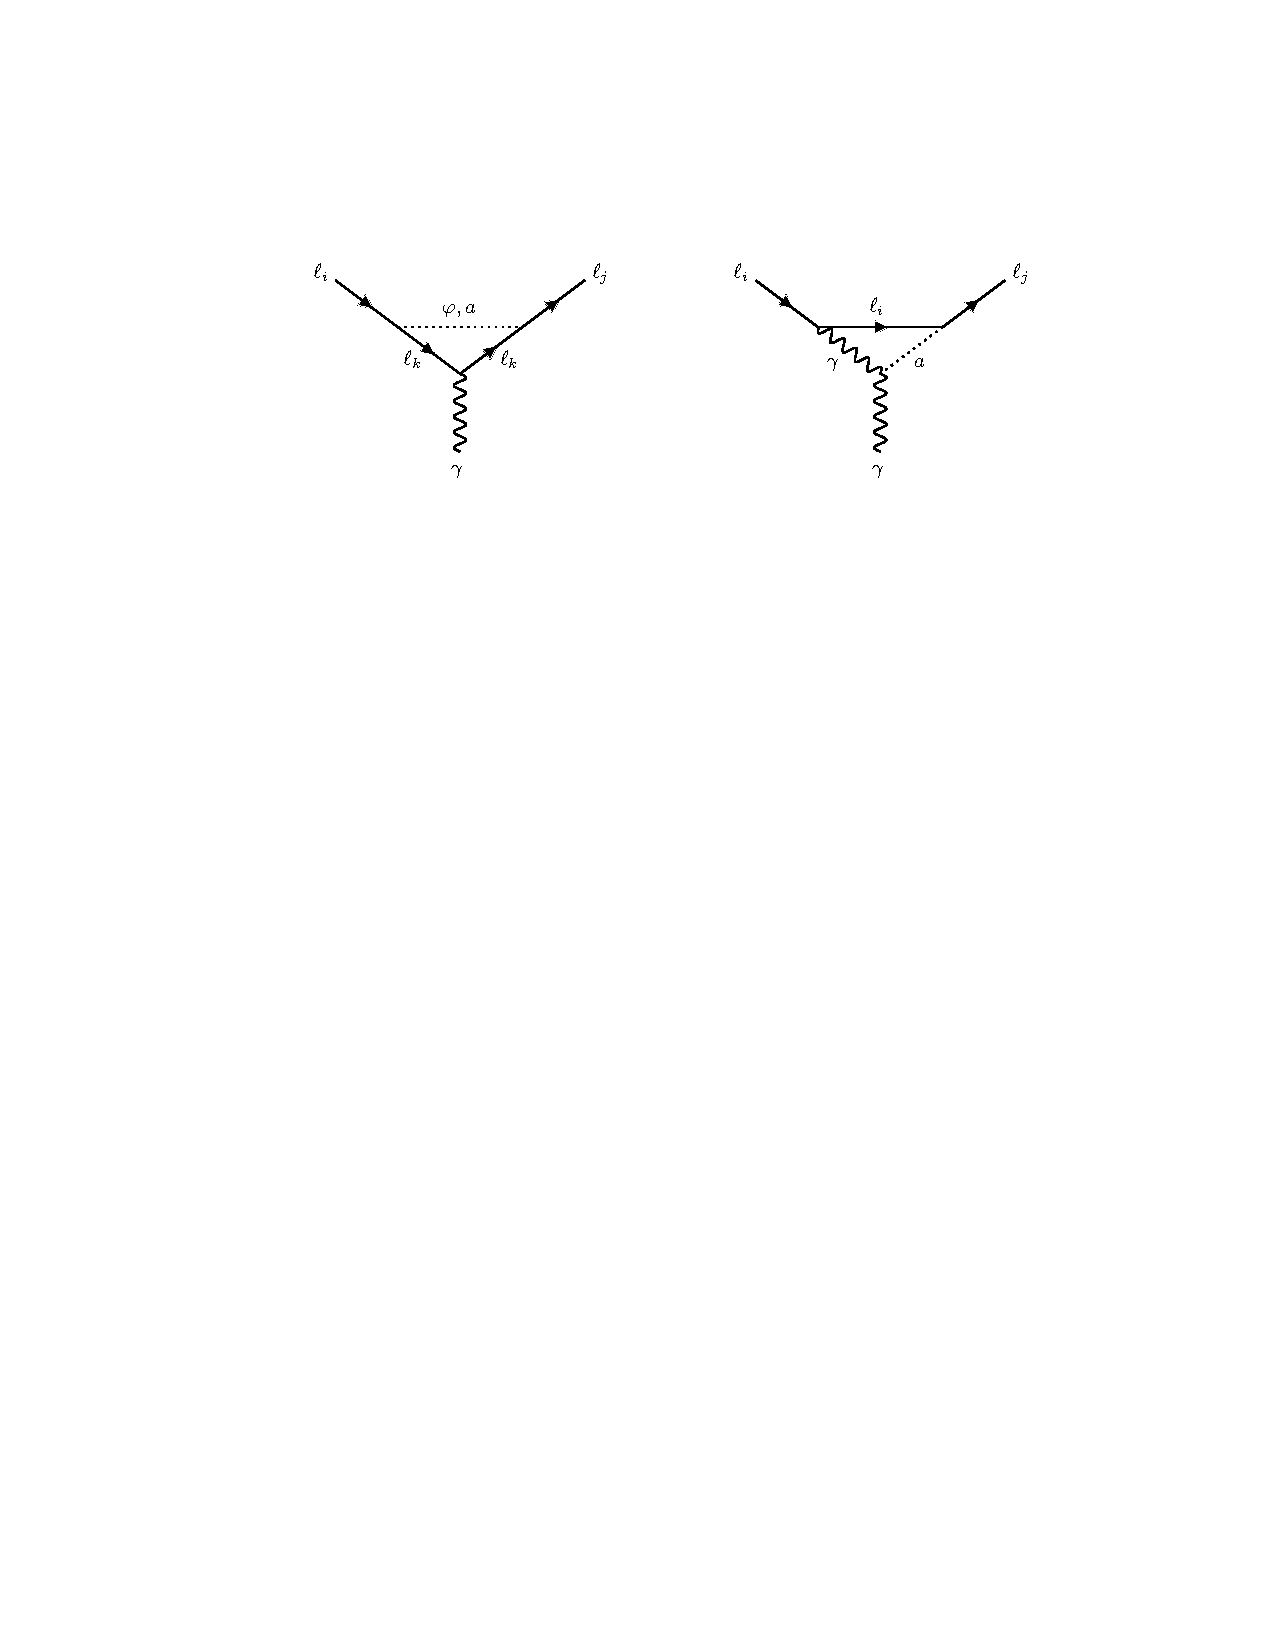
\includegraphics[width=0.9\linewidth]{figures/chapter3/photon_diagram.pdf}
    \caption[Feynman diagrams which contribute to the diagonal and off-diagonal lepton dipole form-factors.]{Feynman diagrams which contribute to the form-factors relevant to the process $\ell_i\rightarrow\ell_j\gamma$, as well as to the lepton dipole moments for $i = j$, for particles with the interaction terms in Eqs.~\ref{eq:LFV_scalar_int} and \ref{eq:LFV_ALP_int}. For leptophilic particles, the right-most diagram only applies to an ALP, which has an induced coupling to photons when rewriting the leptonic interaction to be scalar-like.}
    \label{fig:LFV_vertex}
\end{figure}


The most general gauge-invariant decomposition of the $\ell_i\rightarrow\ell_j$ flavor-changing current into dimensionless form-factors is \cite{Nowakowski:2004cv}
\begin{align}
    \bar{u}_j(q_2)\Gamma^{ij}_\mu u_i(q_1) &= e\bar{u}_j(q_2)\left[\left(q_\mu+\frac{q^2}{m_i - m_j}\gamma_\mu\right) F_1^{ij}(q^2) + \frac{i\sigma^{\mu\nu}}{m_i + m_j}q_\nu F_2^{ij}(q^2)\right. \nonumber\\
    &\ \ \ \ \ \ \ \ \ \ \ \ \ \ \ \ \left. +\frac{\sigma^{\mu\nu}}{m_i - m_j}q_\nu \gamma^5 F_3^{ij}(q^2)+\left(q_\mu-\frac{q^2}{m_i + m_j}\gamma_\mu\right)\gamma^5 F_4^{ij}(q^2)\right]u_i(q_1)
\end{align}
where $\sigma^{\mu\nu} = \tfrac{i}{2}\left[\gamma^\mu,\gamma^\nu\right]$. Here, $F_1(q^2)$ is the charge transition form factor, $F_2(q^2)$ and $F_3(q^2)$ are magnetic and electric dipole transition form-factors, and $F_4(q^2)$ is the anapole transition form-factor. For our purposes, we are only concerned with the dipole transition form-factors evaluated at $q^2 = 0$. Higher $q^2$-dependence and the other form-factors become important when the $\ell_i\rightarrow \ell_j$ transition occurs in loops with an off-shell photon. The only place where this may affect our results is in the loop-induced contribution to $\ell_i \rightarrow \ell_j \ell_k\bar{\ell}_k$ mediated by an off-shell photon. However, in this instance, the bounds from $\ell_i\rightarrow \ell_j\gamma$ are dominant anyway.

We compute the dipole transition form-factors generated by the interactions in Eqs.~\ref{eq:LFV_scalar_int} and \ref{eq:LFV_ALP_as_scalar} by evaluating the left-most Feynman diagram in Fig.~\ref{fig:LFV_vertex}. Using PackageX in Mathematica  \cite{Patel:2016fam}, we find that the exact one-loop form factors at $q^2 = 0$ can be written in the form
\begin{align}
F_2^{ijk}(0) & = \frac{ g_{ik}g_{jk}e^{i\Delta \phi}}{32\pi^2}\left[f(\mu_i, \mu_j, \mu_k)\cos{\theta_{ik}}\cos{\theta_{jk}} + e^{i\Delta \delta}f(-\mu_i, -\mu_j, \mu_k) \sin{\theta_{ik}}\sin{\theta_{jk}}\right]\label{eq:F2ijk}
\intertext{and}
    F_{3}^{ijk}(0) &= \frac{g_{ik}g_{jk}e^{i\Delta \phi}}{32\pi^2}\left[f(-\mu_i, \mu_j, \mu_k)e^{-i\delta_{jk}}\cos{\theta_{ik}}\sin{\theta_{jk}} - f(\mu_i, -\mu_j, \mu_k)e^{i\delta_{ik}}\sin{\theta_{ik}}\cos{\theta_{jk}}\right]\label{eq:F3ijk}
\end{align}
where $\mu_i = m_i/m_\varphi$.\footnote{In the case of a complex scalar, $g_{ij}\neq g_{ji}$ in general, so there is an analogous contribution mediated by the antiparticle which involves the couplings $g_{ki}$ and $g_{kj}$ (and associated phases) as long as they are non-zero.} The function $f$ is given by
\begin{align}
    f(x, y, z) = &\frac{(2z+y)x^2-(2x+y)(z^2+2xz-1)}{(x^2-y^2)x^3}\sqrt{(1-x^2+z^2)^2 - 4z^2}{\rm arccosh}\left(\frac{1-x^2+z^2}{2z}\right)\nonumber\\
    -&\frac{(2z+x)y^2-(2y+x)(z^2+2yz-1)}{(x^2-y^2)y^3}\sqrt{(1-y^2+z^2)^2 - 4z^2}{\rm arccosh}\left(\frac{1-y^2+z^2}{2z}\right)\nonumber\\
    - &\frac{[(x+y)(1-z^2) - xyz]^2 - 3x^2y^2z^2}{x^3y^3}\log z - \frac{1+xy-z^2}{xy}\nonumber\\
    - &\lim_{\varepsilon\rightarrow 0}\int_{0}^1\int_{0}^{1-s}\frac{2(x+y+z)z\,ds\,dt}{x^2 - (x^2-y^2)st+(1-y^2 - z^2)t+y^2t^2 + i\varepsilon},\label{eq:exact_Fijk}
\end{align}
where we are using ${\rm arccosh}\,{u} = \log{(u + \sqrt{u^2 - 1})}$ with the principle branch on the logarithm.\footnote{In Mathematica and NumPy, ${\rm arccosh}\,{u} = \log{(u+\sqrt{u-1}\sqrt{u+1})}$, which leads to an overall sign difference in the real part for $u < -1$. Care must be taken to ensure the proper branch, which is determined by the $\varepsilon$-prescription of the Feynman propagator.} The integral in the last line is a special case of the scalar $C_0$ function obtained through Passarino-Veltman reduction \cite{Passarino:1978jh, Ellis:2011cr}. It can be evaluated in terms of dilogarithms, but one must be careful to choose the branch that corresponds to the $+i{\varepsilon}$ prescription. Note that for pure scalar or pure pseudoscalar couplings, $F_3^{ijk}(0)$ is zero, and only one of the terms involving $f(\pm \mu_i,\pm \mu_j, \mu_k)$ in $F_2^{ijk}(0)$ remains. The pure (pseudo)-scalar scenario is often the focus of works which aim to limit LFV couplings, but as we have seen, the chiral asymmetry of the SM gauge groups can naturally lead to chiral couplings instead.

To explore the chiral scenario, we will consider the special case $\delta_{ik} = \delta_{jk} = \pm\pi/2$, so that the interactions involving the scalar and pseudoscalar currents of each fermion pair have the same phase.\footnote{This is one step away from the CP-preserving scenario, which also requires $\phi_{ik} = \phi_{jk} = 0$.}  This choice encompasses the pure chiral scenario (for which the interaction is proportional to $1 \pm \gamma^5$) but allows for arbitrary PV angles $\theta_{ik}$ and $\theta_{jk}$. In this scenario, it is convenient to define the functions
\begin{align}
    f_{\pm}(\mu_i,\mu_j,\mu_k) = \frac{1}{2}\left[f(\mu_i, \mu_j, \mu_k) \pm f(-\mu_i, -\mu_j, \mu_k)\right].\label{eq:f_plus_minus}
\end{align}
Then, using the reverse cosine and sine product identities, the form-factors can be expressed as
\begin{align}
    F_2^{ijk}(0) = \frac{ g_{ik}g_{jk}e^{i\Delta \phi}}{32\pi^2}&\left(f_-(\mu_i, \mu_j, \mu_k)\cos{(\theta_{ik}+\theta_{jk})}+f_+(\mu_i, \mu_j, \mu_k)\cos{(\theta_{ik}-\theta_{jk})}\right)
\end{align}
and
\begin{align}
    F_3^{ijk}(0) = \pm\frac{ig_{ik}g_{jk}e^{i\Delta \phi}}{32\pi^2}&\left(f_+(\mu_i, -\mu_j, \mu_k)\sin{(\theta_{ik}+\theta_{jk})}-f_-(\mu_i, -\mu_j, \mu_k)\sin{(\theta_{ik}-\theta_{jk})}\right).
\end{align}
At this point, it is customary to expand in the lepton mass hierarchy $m_e \ll m_\mu \ll m_\tau$. For certain processes, this hierarchy can manifest itself within the functions $f_{\pm}$ such that $|f_+| \gg |f_-|$ or $|f_+| \ll |f_-|$, in which case the smaller of the two terms is often neglected. However, this becomes invalid if $\cos{(\theta_{ik}\pm \theta_{jk})}$ or $\sin{(\theta_{ik}\pm \theta_{jk})}$ is also small. Such is the case for a scalar with chiral coupling to the leptons, for which
 $\theta_{ik} = \theta_{jk} = \pm \pi/4$ and hence $\cos(\theta_{ik} + \theta_{jk}) = \sin(\theta_{ik}-\theta_{jk}) = 0$. The form factors are then given by 
\begin{align}
    F_2^{ijk}(0) &= \frac{ g_{ik}g_{jk}e^{i\Delta \phi}}{32\pi^2}f_+(\mu_i, \mu_j, \mu_k),\\
    F_3^{ijk}(0) &= \pm\frac{i g_{ik}g_{jk}e^{i\Delta \phi}}{32\pi^2}f_+(\mu_i, -\mu_j, \mu_k).
\end{align}
Hence, even if $|f_+| \ll |f_-|$, it would be invalid to neglect the terms involving $f_+$, as the terms involving $f_-$ are exactly zero in the chiral case. We will find that this is the case for quite a few of the chiral scalar contributions to the form-factors.

A similar effect can also occur for the ALP, with some important differences. After rewriting the interaction into the form of Eq.~\ref{eq:LFV_ALP_as_scalar}, the difference in lepton masses forces $\theta_{ii} = \pi/2$. Also, for $i\neq j$, $\theta_{ij}$ isn't exactly $\pi/4$, but, assuming $m_i > m_j$, has ${\cal O}(m_j/m_i)$ corrections. Rather than treating these cases separately, we can use the relation { Eq.~\ref{eq:ALP_to_scalar} with $\Theta_{ij} = \pi/4$ and $\Delta_{ij} = \pm\pi/2$ to find
\begin{align}
    F_2^{ijk}(0) &= \pm\frac{ C_{ik}C_{jk}e^{i\Delta \phi}}{32\pi^2}\left[\frac{(m_i+m_j)m_k}{\Lambda^2}f_-(\mu_i, \mu_j, \mu_k)-\frac{m_i m_j + m_k^2}{\Lambda^2}f_+(\mu_i, \mu_j, \mu_k)\right]
\intertext{and}
    F_3^{ijk}(0) &= \pm\frac{ C_{ik}C_{jk}e^{i\Delta \phi}}{32\pi^2}\left[\frac{(m_i-m_j)m_k}{\Lambda^2}f_-(\mu_i, -\mu_j, \mu_k)-\frac{m_i m_j - m_k^2}{ \Lambda^2}f_+(\mu_i, -\mu_j, \mu_k)\right].
\end{align}
In this case, most of the $\ell_i \rightarrow \ell_j$ dipole form factors are insensitive to the difference between pure and chiral couplings. However, there are still significant differences between the chiral and pure pseudoscalar scenarios for the $\mu \stackrel{\tau}{\longrightarrow}e\gamma$ decay mode, which (all couplings equal) happens to produce the strongest limits of all the decay modes. 

Finally, we must address the additional photonic coupling in the case of the ALP. This can generate the diagram on the right of Fig.~\ref{fig:LFV_vertex}. Rather than provide an exact expression, we use an expression which is valid for $m_i \gg m_j$  \cite{Cornella:2019uxs}
\begin{align}
    F_2^{ij\gamma}(0) &= -\frac{\alpha A_{ij}\sum_\ell A_{\ell\ell}}{16\pi^3}\frac{m_i^2}{\Lambda^2}\left[2\log\frac{\Lambda^2}{m_i^2} + 2 + (x_i-1)\log{(x_i-1)}-\frac{x_i^2}{x_i-1}\log{x_i}\right]\\
    F_3^{ij\gamma}(0) &= -\frac{i\alpha V_{ij}\sum_\ell A_{\ell\ell}}{16\pi^3}\frac{m_i^2}{\Lambda^2}\left[2\log\frac{\Lambda^2}{m_i^2} + 2 + (x_i-1)\log{(x_i-1)}-\frac{x_i^2}{x_i-1}\log{x_i}\right].
\end{align}
Neglecting interference with diagrams involving the other form-factors, we will find that the $\ell_i \rightarrow \ell_j\gamma$ and $\ell_i \rightarrow \ell_j\ell_k \bar{\ell}_l$ decay rate mediated by the fermion-loop-induced photonic coupling are proportional to $|A_{ij}|^2 + |V_{ij}|^2 = C_{ij}^2$, and are hence independent of PV in the interaction.

\subsection{Approximations}\label{sec:transition_approx}

Here we will cite approximate formulae for $f_{\pm}$ for the relevant hierarchies of $m_i$, $m_j$, and $m_k$. These formulae appear to match the exact results within $10\%$ over almost all ranges of parameters, with especially good agreement for $m_a > m_i$. For easy comparison with other results in the literature, we rewrite the functions in terms of $x_i = m_\varphi^2/m_i^2 = 1/\mu_i^2$. Not only are these formulae useful for examining the effect of chiral interactions, but they are also useful for avoiding floating-point errors when numerically evaluating Eq.~\ref{eq:exact_Fijk}.

\begin{enumerate}
    \item $i = k > j$\\
    This regime is relevant for $\mu \rightarrow e\gamma$ with an internal $\mu$, and $\tau \rightarrow e\gamma$ and $\tau \rightarrow \mu \gamma$ with an internal $\tau$. In the limit $m_i \gg m_j$,
        \begin{align}
        f_+(\mu_i,\mu_j,\mu_k) &= 2x_i-3 - (x_i - 3)x_i\log{x_i} + 2(x_i-1)\sqrt{x_i(x_i - 4)}\log\left(\frac{x_i+\sqrt{x_i(x_i - 4)}}{2\sqrt{x_i}}\right) \nonumber\\
        &\ - \log^2\left(\frac{x_i+\sqrt{x_i(x_i-4)}}{2x_i}\right) - 2{\rm Li}_2\left(1-x_i\right)\nonumber\\
        & - 2{\rm Li}_2\left(\frac{x_i - \sqrt{x_i(x_i-4)}}{2x_i}\right) + 2{\rm Li}_2\left(\frac{2-x_i - \sqrt{x_i(x_i-4)}}{2}\right),\nonumber\\
        f_-(\mu_i,\mu_j,\mu_k) &=-2 + \frac{(x_i - 3)x_i}{x_i-1}\log{x_i} - 2\sqrt{x_i(x_i - 4)}\log\left(\frac{x_i+\sqrt{x_i(x_i - 4)}}{2\sqrt{x_i}}\right)\nonumber\\
        &\ - \log^2\left(\frac{x_i+\sqrt{x_i(x_i-4)}}{2x_i}\right) - 2{\rm Li}_2\left(1-x_i\right)\nonumber\\
        & - 2{\rm Li}_2\left(\frac{x_i - \sqrt{x_i(x_i-4)}}{2x_i}\right) + 2{\rm Li}_2\left(\frac{2-x_i - \sqrt{x_i(x_i-4)}}{2}\right).
        \end{align}
        The terms involving the dilogarithms are identical for both $f_+$ and $f_-$, and hence cancel for the pure pseudoscalar amplitude (for which the surviving part of the form factor is $f(-\mu_i, -\mu_j, \mu_k) = f_+(\mu_, \mu_j, \mu_k) - f_-(\mu_i, \mu_j, \mu_k)$). In this case, any significant differences between the pure scalar scenario and chiral scenario are due solely to differences in the functional form of $f_+$ and $f_-$, as there is no explicit lepton mass ratio appearing in either of the functions. Nevertheless, the final results in Fig.~\ref{fig:LFV_limits}  show that the difference in functional forms is enough to induce a substantial difference between the pure-scalar and chiral couplings.
        
    \item $i > j,k$\\
    This regime is relevant for $\tau \rightarrow \mu \gamma$ and $\tau \rightarrow e\gamma$, with an internal $\mu$ or $e$. In the limit $m_\tau \gg m_\mu, m_e$, we have
    \begin{align}
    f_+(\mu_i, \mu_j, \mu_k) &= -1+2x_i + 2(x_i - 1)x_i \log\left(\frac{x_i - 1}{x_i}\right)\nonumber\\
    f_-(\mu_i, \mu_j, \mu_k) &= \frac{2\mu_k}{\mu_i}\left[ \left(1 - x_i -\log\left(\frac{(x_i-1)x_k}{x_i}\right)\right)\log\left(\frac{x_i-1}{x_i}\right) - {\rm Li}_2\left(\frac{1}{x_i}\right) - 1\right].
    \end{align}
    The second term is often neglected compared to the first in the $m_k / m_i$ expansion, but we note that this is not valid in the case of $\tau \overset{\mu}{\longrightarrow} \ell\gamma$. In particular, even though $\mu_\tau/\mu_\mu = m_\mu/m_\tau \approx 0.06$, $|f_-| > |f_+|$ for almost all $x_\tau > 1$. Hence, similar to case (1), differences in the functional forms of $f_{\pm}$ are enough to induce differences in the pure-scalar and chiral cases for $\tau\rightarrow\mu\gamma$, which is apparent in the second and third panels of Fig.~\ref{fig:LFV_limits}. (Although not particularly relevant for the masses we consider, we note that for $x_i < 1$, one should choose the branch $\log{(x)} = -i\pi + \log{(-x)}$.)
    
    \item $k > i, j$\\
    This regime is relevant for $\mu \rightarrow e\gamma$ with an internal $\tau$. In the limit $m_\tau \gg m_\mu, m_e$, we have
    \begin{align}
    f_+(\mu_i, \mu_j, \mu_k) &= \left(\frac{\mu_i + \mu_j}{\mu_k}\right)^2\left[\frac{2x_k^2 + 5x_k - 1}{6(x_k - 1)^3}-\frac{x_k^2}{(x_k-1)^4}\log{x_k}\right], \nonumber\\
f_-(\mu_i, \mu_j, \mu_k) &= \frac{\mu_i + \mu_j}{\mu_k}\left[-\frac{3x_k - 1}{(x_k - 1)^2} + \frac{2x_k^2}{(x_k-1)^3}\log{x_k}\right].
    \end{align}
    Typically, only the functional form in $f_-$ is cited, because $(m_\mu + m_e)/m_\tau \ll 1$. Unlike in case (2) for $\tau\rightarrow\mu\gamma$, this approximation is valid, and $|f_+| \ll |f_-|$ for large $m_\varphi$. As discussed before, only $f_+$ contributes for chiral interactions, so the contribution of a chiral scalar to $\mu\stackrel{\tau}{\longrightarrow}e\gamma$ is massively suppressed compared to the contribution of a pure scalar, as seen in the first panel of Fig.~\ref{fig:LFV_limits}. This is also apparent (though to a lesser extent) for ALPs, as seen in Fig.~\ref{fig:LFV_limits}.
\end{enumerate}
The approximate functional forms for cases (1)-(3) are in agreement with those found in Refs.~\cite{Escribano:2020wua,Cornella:2019uxs,Bauer:2021mvw}, but include additional terms that may be relevant depending on the PV nature of the interaction. Apart from these results for lepton mass hierarchies, we can also derive a general result when $m_\varphi$ is large ($\mu_i, \mu_j, \mu_k \ll 1$). Then, the form-factor function takes on the simplified form
\begin{align}
    f(\mu_i, \mu_j, \mu_k) = (\mu_i+\mu_j)\left(\frac{\mu_i+\mu_j}{3} - 3\mu_k - 4\mu_k \log{\mu_k}\right).
\end{align}
So in particular, $f_+(\mu_i, \mu_j, \mu_k) \approx (\mu_i+\mu_j)^2$ and $f_-(\mu_i, \mu_j, \mu_k) \approx -(\mu_i+\mu_j)(3\mu_k+4\mu_k\log{\mu_k})$. This formula is only accurate when $m_\varphi$ is very large, so is only relevant at the right-most end of the plots in Fig.~\ref{fig:LFV_limits}.

\subsection{Radiative Decay}\label{sec:radiative}
Now, we are ready to place limits from LFV lepton decays, beginning with the radiative decay $\ell_i \rightarrow \ell_j\gamma$. The spin-averaged decay rate for $\ell_i \rightarrow \ell_j\gamma$ is given by
\begin{align}
    \Gamma(\ell_i\rightarrow\ell_j\gamma) &= \frac{\alpha_{\rm em}}{2}\left(\frac{(m_i - m_j)^2}{ m_i}\left|F_2^{ij}(0)\right|^2 + \frac{(m_i + m_j)^2}{ m_i}\left|F_3^{ij}(0)\right|^2\right).
\end{align}
These decay modes have been searched for extensively in particle physics experiments, as observation of such an event would be smoking-gun evidence of new physics. The Mu E Gamma (MEG) experiment, which ran from 2009 to 2013, constrained the branching fraction for $\mu \rightarrow e\gamma$ by ${\cal B}(\mu \rightarrow e\gamma) < 4.2\times 10^{-13}$ at the 90\% confidence level \cite{Mori:2016vwi}. More recently, the first results from the upgrade, MEG II, have improved these results to ${\cal B}(\mu \longrightarrow e\gamma) < 3.1 \times 10^{-13}$ \cite{MEGII:2023ltw}. By the end of its run in 2026, MEG II expects to improve the sensitivity to $\lesssim 6\times 10^{-14}$ \cite{MEGII:2018kmf}.
\begin{table}[t!]
\centering
\begin{tabular}{|c|cc|cc|}
\hline
\multirow{2}{*}{\rule{0pt}{2.5ex}Process}   & \multicolumn{2}{c|}{Constraints}                                 & \multicolumn{2}{c|}{Projections}                                 \\ \cline{2-5} 
                           & \multicolumn{1}{c|}{Experiment} & ${\cal B}$ limit (90\% CL) & \multicolumn{1}{c|}{Experiment} & ${\cal B}$ limit (90\% CL) \\ \hline
\rule{0pt}{2.5ex}$\mu \rightarrow e\gamma$   & \multicolumn{1}{c|}{MEG, MEG II} & $~~<3.1\times10^{-13}$\cite{MEGII:2023ltw}\,\, & \multicolumn{1}{c|}{MEG II} & $\,\,\lesssim 6\times10^{-14}$\cite{MEGII:2018kmf}\,\,\,\\
$\tau\rightarrow e\gamma$  & \multicolumn{1}{c|}{BaBar} & $<3.3\times10^{-8}$\cite{BaBar:2010axs} & \multicolumn{1}{c|}{Belle II} & $\lesssim 9\times10^{-9}$\cite{Belle-II:2018jsg}\,\,\,\\
$\tau\rightarrow\mu\gamma$ & \multicolumn{1}{c|}{Belle} & $~\,<4.2\times10^{-8}$ \cite{Belle:2021ysv}\,& \multicolumn{1}{c|}{Belle II} & $\lesssim 7\times10^{-9}$\cite{Belle-II:2018jsg} \,\\
$\mu\rightarrow ee\bar{e}$ & \multicolumn{1}{c|}{SINDRUM} & \,\,$<1.0\times10^{-12}$\cite{SINDRUM:1987nra} & \multicolumn{1}{c|}{Mu3e} & $\lesssim 2\times10^{-15}$\cite{Mu3e:2020gyw}\\ 
$\tau\rightarrow ee\bar{e}$       & \multicolumn{1}{c|}{Belle} & $<2.7\times10^{-8}$\cite{Hayasaka:2010np} & \multicolumn{1}{c|}{Belle II} & $\lesssim 5\times10^{-10}$\cite{Belle-II:2018jsg} \\
$\tau\rightarrow ee\bar{\mu}$     & \multicolumn{1}{c|}{Belle} & $<1.5\times10^{-8}$\cite{Hayasaka:2010np} & \multicolumn{1}{c|}{Belle II} & $\lesssim 3\times10^{-10}$\cite{Belle-II:2018jsg} \\ 
$\tau\rightarrow e\mu\bar{e}$     & \multicolumn{1}{c|}{Belle} & $<1.8\times10^{-8}$\cite{Hayasaka:2010np} & \multicolumn{1}{c|}{Belle II} & $\lesssim 3\times10^{-10}$\cite{Belle-II:2018jsg} \\ 
$\tau\rightarrow \mu\mu\bar{\mu}$ & \multicolumn{1}{c|}{Belle} & $<2.1\times10^{-8}$\cite{Hayasaka:2010np} & \multicolumn{1}{c|}{Belle II} & $\lesssim 4\times10^{-10}$\cite{Belle-II:2018jsg} \\ 
$\tau\rightarrow \mu e\bar{\mu}$  & \multicolumn{1}{c|}{Belle} & $<2.7\times10^{-8}$\cite{Hayasaka:2010np} & \multicolumn{1}{c|}{Belle II} & $\lesssim 5\times10^{-10}$\cite{Belle-II:2018jsg} \\ 
$\tau\rightarrow \mu \mu\bar{e}$  & \multicolumn{1}{c|}{Belle} & $<1.7\times10^{-8}$\cite{Hayasaka:2010np} & \multicolumn{1}{c|}{Belle II} & $\lesssim 3\times10^{-10}$\cite{Belle-II:2018jsg} \\ 
\hline
\end{tabular}\label{table:LFV_decay_limits}
\caption{Current experimental constraints and future prospects on the branching fractions for the decay modes $\ell_i \rightarrow \ell_j\gamma$ and $\ell_i \rightarrow \ell_j\ell_k\bar{\ell}_l$ at the 90\% confidence level.}
\end{table}
There have also been less stringent limits placed on the $\tau\rightarrow \ell\gamma$ decays by the the BaBar experiment at SLAC and the Belle experiment at KEK-B. The BaBar experiment achieved an upper limit on the $\tau \rightarrow \ell \gamma$ branching fraction of ${\cal B}(\tau \rightarrow e\gamma) < 3.3\times 10^{-8}$ and ${\cal B}(\tau \rightarrow \mu\gamma) < 4.4\times 10^{-8}$ at the 90\% confidence level \cite{BaBar:2010axs}. More recently, the Belle experiment has reported upper limits at the 90\% confidence level of ${\cal B}(\tau \rightarrow e\gamma) < 5.6\times 10^{-8}$ and ${\cal B}(\tau \rightarrow \mu\gamma) < 4.2\times 10^{-8}$ \cite{Belle:2021ysv}, slightly improving the $\tau \rightarrow \mu \gamma$ result from BaBar. These results are expected to be superceded by Belle II, which aims to achieve a sensitivity of ${\cal B}(\tau \rightarrow e\gamma) \lesssim 9\times 10^{-9}$ and ${\cal B}(\tau \rightarrow \mu\gamma) \lesssim 7\times 10^{-9}$ by the year 2030 \cite{Banerjee:2022vdd}. A summary of these radiative decay limits is shown in Table \ref{table:LFV_decay_limits}.

\subsection{Trilepton Decay}\label{sec:trilepton}

\begin{figure}[t!]
    \centering
    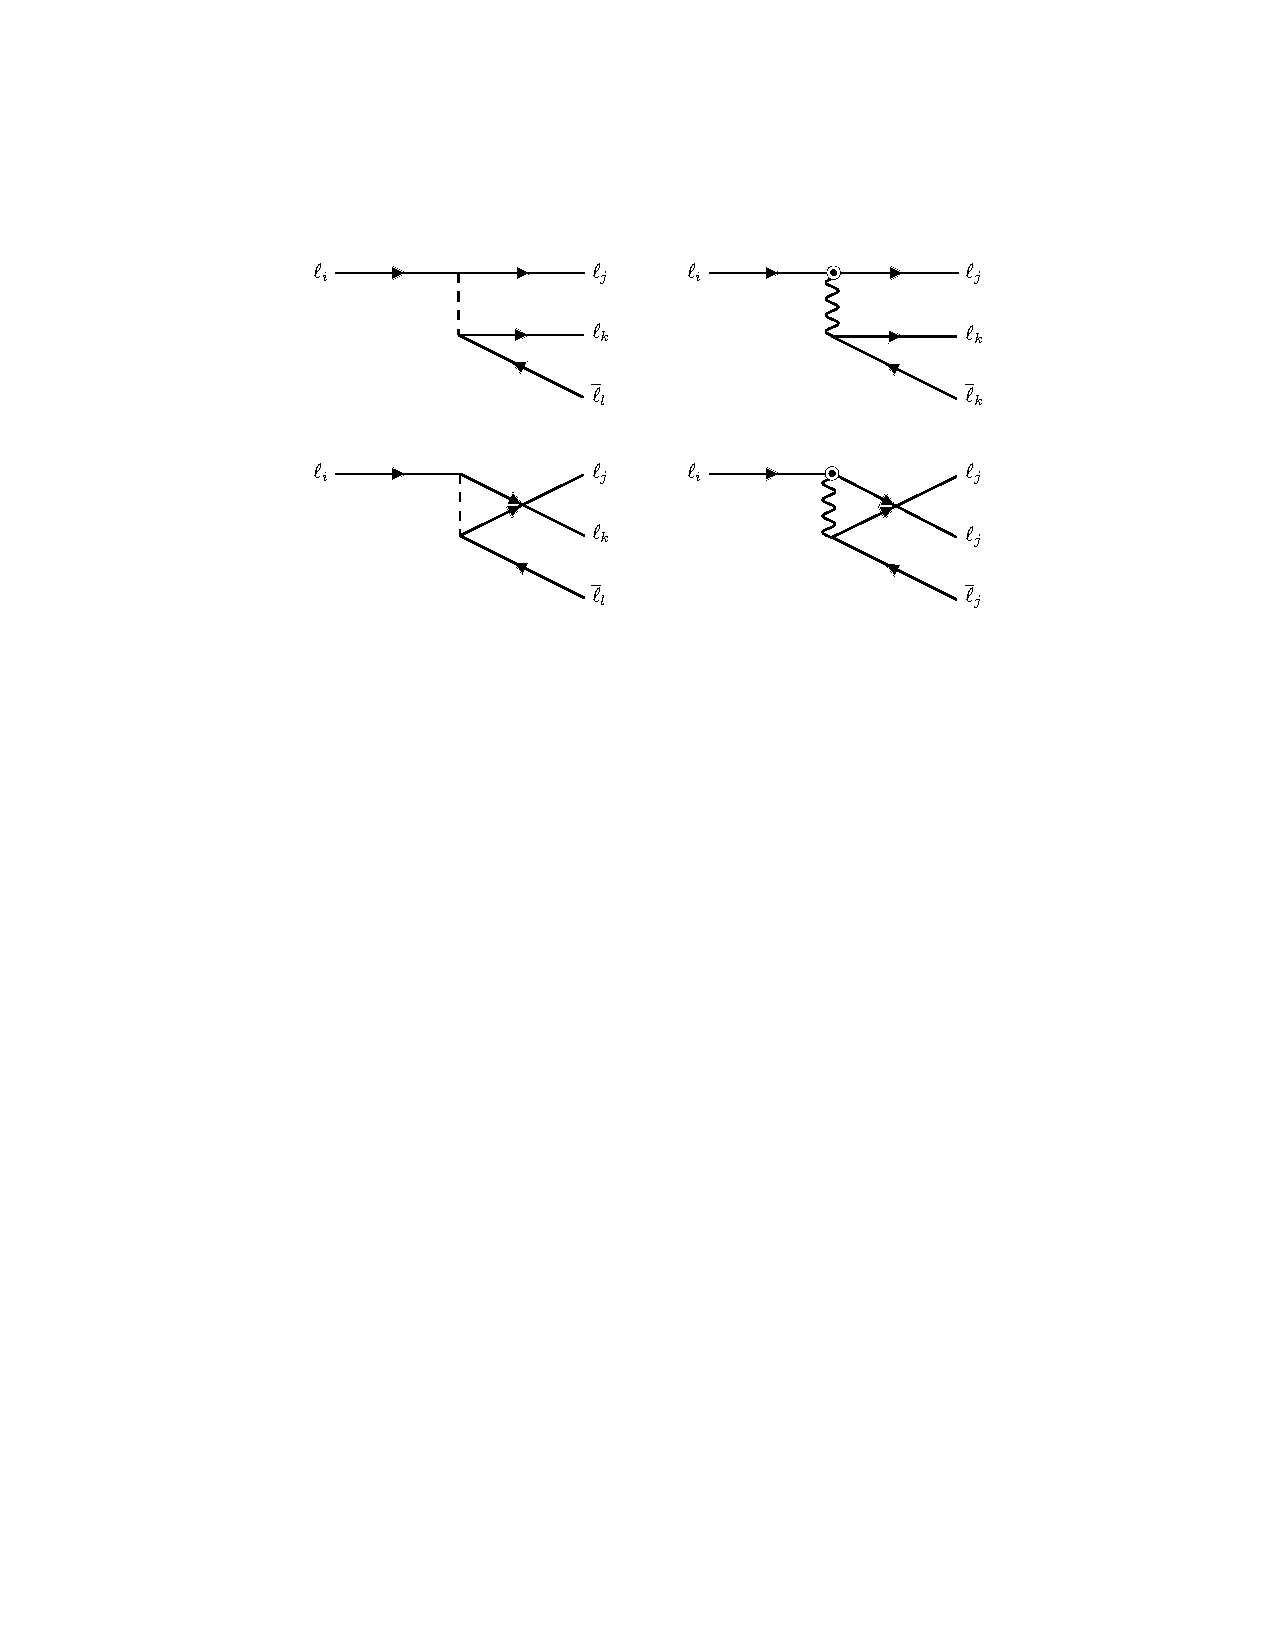
\includegraphics[width=0.8\linewidth]{figures/chapter3/trilepton_diagram.pdf}
    \caption[Feynman diagrams which contribute to the trilepton decay processes $\ell_i \rightarrow \ell_j \ell_k \bar{\ell}_l$. ]{Feynman diagrams which contribute to the trilepton decay processes $\ell_i \rightarrow \ell_j \ell_k \bar{\ell}_l$.  For light $\varphi$, the left-most diagrams dominate, whereas for heavy $\varphi$ the left and right can be comparable in size.}
    \label{fig:trilepton_vertex}
\end{figure}

Now, we turn to the trilepton decay modes $\ell_i \rightarrow \ell_j \ell_k\bar{\ell}_l$, depicted in Fig.~\ref{fig:trilepton_vertex}. There are two main subprocesses: mediation via an off-shell $\varphi$ ($\ell_i\rightarrow\ell_j\varphi^*(\varphi^*\rightarrow \ell_k\bar{\ell}_k))$ and (for $l = k$) via the transition lepton dipole moment and an off-shell photon ($\ell_i \rightarrow \ell_j\gamma^*(\gamma^*\rightarrow \ell_k \bar{\ell}_k))$. We will not concern ourselves with interference between these diagrams. Rather than computing the dipole transition contribution directly, we estimate
\begin{align}
    \Gamma(\ell_i \longrightarrow \ell_j \ell_k\bar{\ell}_k) &\approx \frac{\alpha}{3\pi}\left(\log\frac{m_i^2}{m_k^2}-3 + \frac{\delta_{jk}}{4}\right)\Gamma(\ell_i \rightarrow \ell_j \gamma)
\end{align}
in line with Refs. \cite{Abada:2014kba, Cornella:2019uxs} (ignoring contributions from the anapole form-factors). While this term is typically subdominant for scalars, it can be dominant depending on the relative strengths of the couplings. For ALPs, it is typically dominant when $\ell_k = e$, because the analogous contribution from an off-shell ALP involves an $ee$ coupling which is suppressed to $m_e^2/\Lambda^2$. Given that the coefficient is suppressed by $\alpha/3\pi$, we expect that when this diagram is the main contribution to the trilepton decay rate, the corresponding limits from $\ell_i\rightarrow\ell_j\gamma$ are stronger.

Defining $s_{ij} \equiv (p_i - p_j)^2 = 4p_k^2$ and $s_{ik} \equiv (p_i - p_k)^2 = (p_j+p_k)^2$, we find that the $\ell_i \rightarrow \ell_j\ell_k\bar{\ell}_l$ amplitude is given by
\begin{align}
    \overline{\left|{\cal M}\right|^2} &= 2g_{ij}^2g_{kl}^2\frac{[m_{ij}^2(\theta_{ij}) - s_{ij}][s_{ij}-m_{kl}^2(\theta_{kl})]}{(m_\varphi^2 - s_{ij}^2)^2}\nonumber\\
    &\ + 2g_{ik}^2g_{jl}^2\frac{[m_{ij}^2(\theta_{ik}) - s_{ik}][s_{ik}-m_{jl}^2(\theta_{jl})]}{(m_\varphi^2-s_{ik}^2)^2}\nonumber\\
    &\ +4g_{ij}g_{kl}g_{ik}g_{jl}\frac{s_{ij}s_{ik}}{(m_\varphi^2-s_{ij})(m_\varphi^2-s_{ik})}{\cal S}_{ijkl}
\end{align}
where $m_{ij}^2(\theta) = m_i^2+m_j^2 + 2m_im_j\cos{2\theta}_{ij}$ and we have defined
\begin{align}
    {\cal S}_{ijkl} = \frac{1}{2}{\rm Re}\{&e^{i\Phi}U(\theta_{ij},\delta_{ij})\overline{U}(\theta_{jk},\delta_{jk})U^*(\theta_{ik},\delta_{ik})\overline{U}^*(\theta_{kl},\delta_{kl})\nonumber\\
   +&e^{i\Phi}\overline{U}(\theta_{ij},\delta_{ij})U(\theta_{jk},\delta_{jk})\overline{U}^*(\theta_{ik},\delta_{ik})U^*(\theta_{kl},\delta_{kl})\}
\end{align}
with $\Phi = \phi_{ij}-\phi_{ik}+\phi_{jl}-\phi_{kl}$ and
\begin{align}
    U(\theta,\delta) \equiv \cos{\theta}+ie^{i\delta}\sin{\theta},\ \ \overline{U}(\theta,\delta) \equiv \cos{\theta}-ie^{i\delta}\sin{\theta}.
\end{align}
We can see immediately that the size of the interference term is strongly dependent on both the PV and CPV nature of the $\varphi$ couplings. In the event that all $\theta_{ij} \equiv \theta$ and $\delta_{ij} \equiv \delta$, we have $|{\cal M}|^2_{\rm int} \propto 1-\sin^2{2\theta}\sin^2{\delta}$. In particular, for chirally coupled particles ($\theta = \pi/4$, $\delta = \pi/2$), the interference term goes to zero. This is in contrast to the diagonal terms, which are only affected by the PV angle at ${\cal O}(m_j/m_i)$ or ${\cal O}(m_k/m_i)$. 


Ignoring the width of the $\varphi$ and using $m_j, m_k, m_l \ll m_i$, we find that the decay rate is given by
\begin{align}
    \Gamma(\ell_i \rightarrow \ell_j \ell_k \overline{\ell}_l) &= \frac{1}{\sigma_{jk}}\frac{1}{32\pi^2}\int{ds_{ij}ds_{ik}\Theta(s_{ik}-(m_k - m_l)^2)\Theta((m_i+m_j)^2-s_{ik})|{\cal M}|^2}\nonumber\\
    &\approx \frac{1}{\sigma_{jk}}\frac{m_i}{512\pi^3}\left[(g_{ij}^2g_{kl}^2+g_{ik}^2g_{jl}^2)h_1(x_i) + 2g_{ij}g_{jl}g_{ik}g_{kl}{\cal S}_{ijkl}h_2(x_i)\right]
\end{align}
where $x_i = m_\varphi^2/m_i^2$, $\sigma_{jk} = 1 + \delta_{jk}$ is a symmetry factor, and
\begin{align}
    h_1(x) &= -5 + 6x-2(1-4x+3x^2)\log\frac{x}{x-1}\\
    h_2(x) &= 2-8x-\frac{2\pi^2}{3}x^2+8(x-1)x\log\frac{x}{x-1}+4x^2\log^2\frac{x}{2x-1}+8x^2{\rm Li}_2\left(\frac{x}{2x-1}\right).
\end{align}
These functions are in agreement with those found in Ref.~\cite{Cornella:2019uxs} for ALP-mediated processes. In particular, $h_1(x) \approx h_2(x) \approx 1/12x^2$ for large $x$, so (assuming ${\cal S}_{ijkl} = 1$)
\begin{align}
\Gamma(\ell_i \rightarrow \ell_j \ell_k \overline{\ell}_l) &\approx \frac{1}{\sigma_{jk}}\frac{m_i^5}{6144\pi^3m_\varphi^4}(g_{ij}g_{kl} + g_{ik}g_{jl})^2.
\end{align}
This is in agreement with  Ref.~\cite{Dev:2017ftk}, which studies such decays mediated by LFV neutral scalars. This expression is valid when the $\varphi$ is heavy and its width can be ignored. For $m_\varphi < m_i$, the width becomes important. In this case, one can use the narrow width approximation
\begin{align}
    \Gamma(\ell_i \rightarrow \ell_j\ell_k\bar{\ell}_l) &= \Gamma(\ell_i\rightarrow \ell_j\varphi){\cal B}(\varphi\rightarrow \rightarrow \ell_k\bar{\ell}_l)+\Gamma(\ell_i\ell_k\varphi){\cal B}(\varphi \rightarrow \ell_j\bar{\ell}_l)
\end{align}
with 
\begin{align}
    \Gamma(\ell_i\rightarrow \ell_j\varphi) = g_{ij}^2\frac{m_i}{16\pi}\left(1-\frac{m_\varphi^2}{m_i^2}\right)^2
\end{align}
and
\begin{align}
\Gamma(\varphi\rightarrow \ell_i\bar{\ell}_j) = g_{ij}^2\frac{m_\varphi}{8\pi}\left(1 - \frac{m_{ij}^2(\theta_{ij})}{m_\varphi^2}\right)\sqrt{\left(1- \frac{(m_i + m_j)^2}{m_\varphi^2}\right)\left(1- \frac{(m_i - m_j)^2}{m_\varphi^2}\right)}.
\end{align}
Like the radiative decays in the previous section, the branching fractions for these trilepton decay modes are highly constrained by modern particle physics experiments. The leading limit on $\mu\rightarrow e e\bar{e}$ has remained the same since 1988, when the SINDRUM experiment found it to be ${\cal B}(\mu \rightarrow ee\bar{e}) < 1.0\times 10^{-12}$ at the 90\% confidence level \cite{SINDRUM:1987nra}. All of the leading limits on ${\cal B}(\tau \rightarrow 3\ell)$ come from the Belle experiment, ranging from $1.7\times 10^{-8}$ to $2.7\times 10^{-8}$ at the 90\% confidence level \cite{Hayasaka:2010np}. The Belle II experiment is expected to improve these bounds to between $3\times10^{-10}$ and $5\times10^{-10}$ by 2030.  A summary of all the trilepton branching limits and projections is shown in Table~\ref{table:LFV_decay_limits}.

\begin{table}[t!]
\vspace{0.5cm}
\centering
\resizebox{\textwidth}{!}{
\begin{tabular}{@{}ccccccccccccc@{}}
\toprule
Process & $g_{ee}g_{e\mu}$  & $g_{\mu\mu}g_{e\mu}$ & $g_{\tau\tau}g_{e\mu}$ & $g_{e\tau}g_{\mu\tau}$ & $g_{ee}g_{e\tau}$ & $g_{\mu\mu}g_{e\tau}$ & $g_{\tau\tau}g_{e\tau}$ & $g_{e\mu}g_{\mu\tau}$ & $g_{ee}g_{\mu\tau}$ & $g_{\mu\mu}g_{\mu\tau}$  & $g_{\tau\tau}g_{\mu\tau}$ & $g_{e\mu}g_{e\tau}$ \\ \bottomrule \midrule
$\mu\rightarrow e\gamma$ & \ccmark & \ccmark & \cemark & \ccmark & \cxmark &\cxmark & \cxmark  & \cxmark & \cxmark & \cxmark & \cxmark & \cxmark \\ \midrule
$\mu \rightarrow ee\bar{e}$ & \ccmark & \lcmark & \lemark & \lcmark & \cxmark & \cxmark & \cxmark & \cxmark  & \cxmark & \cxmark & \cxmark & \cxmark  \\ \bottomrule \midrule
$\tau\rightarrow e\gamma$ & \cxmark & \cxmark & \cxmark & \cxmark & \ccmark & \cemark & \ccmark & \ccmark & \cxmark & \cxmark & \cxmark & \cxmark  \\ \midrule
$\tau \rightarrow ee\bar{e}$ & \cxmark & \cxmark & \cxmark & \cxmark & \ccmark & \lemark & \lcmark  & \lcmark  & \cxmark  & \cxmark  & \cxmark & \cxmark  \\ \midrule
$\tau \rightarrow e\mu \bar{\mu}$ & \cxmark & \cxmark & \cxmark & \cxmark & \lcmark & \ccmark & \lcmark & \ccmark & \cxmark & \cxmark & \cxmark & \cxmark \\ \bottomrule \midrule
$\tau\rightarrow \mu\gamma$ & \cxmark & \cxmark & \cxmark & \cxmark & \cxmark & \cxmark & \cxmark & \cxmark & \cemark & \ccmark & \ccmark & \ccmark  \\ \midrule
$\tau \rightarrow \mu e\bar{e}$  & \cxmark & \cxmark & \cxmark & \cxmark & \cxmark & \cxmark & \cxmark & \cxmark & \ccmark & \lcmark & \lcmark & \ccmark  \\ \midrule
$\tau \rightarrow \mu\mu\bar{\mu}$ & \cxmark & \cxmark & \cxmark & \cxmark & \cxmark & \cxmark & \cxmark & \cxmark & \lemark  & \ccmark  & \lcmark & \lcmark \\ \bottomrule \midrule 
$\tau \rightarrow ee\bar{\mu}$ & \cxmark & \cxmark & \cxmark & \cxmark & \cxmark & \cxmark & \cxmark & \cxmark & \cxmark  & \cxmark & \cxmark & \ccmark \\ \midrule
$\tau \rightarrow \mu\mu\bar{e}$ & \cxmark & \cxmark & \cxmark & \cxmark & \cxmark & \cxmark & \cxmark & \ccmark & \cxmark  & \cxmark & \cxmark & \cxmark \\ \bottomrule \midrule
\end{tabular}
}


\caption[A table demonstrating which LFV coupling products contribute to each LFV lepton decay.]{A table demonstrating which coupling products contribute to each process. A green check-mark (\ccmark) indicates the product $g_{ij}g_{kl}$ contributes to the process, whereas a red X-mark (\cxmark) indicates it does not. Orange exclamation marks (\cemark) indicate that the process is only sensitive to leptophilic ALPs (per the induced photon coupling), not leptophilic scalars. Light green check-marks (\lcmark) and light orange exclamation marks (\lemark) for the trilepton decay modes $\ell_i\rightarrow \ell_j \ell_k\overline{\ell}_k$ indicate that the process only occurs due to the corresponding dipole transition $\ell_i \rightarrow \ell_j \gamma$, and so the branching for these processes through these couplings is suppressed compared to the $\ell_i \rightarrow \ell_j\gamma$ process.}
\label{table:coupling_products}
\end{table}

\subsection{Limits from LFV Decays}\label{sec:lfv_limits}

Now we present limits on the scalar and ALP interactions from Section \ref{sec:lfv_eft}. Each of these processes requires two distinct couplings to occur, so we place limits on the coupling products $\sqrt{g_{ij}g_{kl}}$ and $\sqrt{C_{ij}C_{kl}}/\Lambda$ under the assumption that all couplings which don't enter the product are zero. A summary of the relevant coupling products for each LFV decay mode is shown in Table~\ref{table:coupling_products}. While generic scalar and ALP models will typically have more than two non-zero couplings, limits of this form illustrate which couplings are the most sensitive to each processes, and limits on models with more complicated hierarchies can in-principle be derived from these limits. 

We begin with limits on pure scalars (solid lines) and chiral scalars (dashed lines) in the top of Fig.~\ref{fig:LFV_limits}. Darker shades represent limits from the radiative decay modes, whereas lighter shades represent limits from the trilepton decay modes. We find that while the trilepton decay limits are largely unaffected by the presence of chiral couplings, the radiative decay limits on chiral scalars are substantially suppressed compared to the limits on pure scalars. The effect is most drastic for the $\mu\overset{\tau}{\longrightarrow} e\gamma$ decay mode, for which $\sqrt{g_{\mu\tau}g_{e\tau}}$ is reduced by an order of magnitude for the chiral scalar. This corresponds to a factor of $10^4$ in the decay rate. 


\begin{figure}[t!]
    \centering
    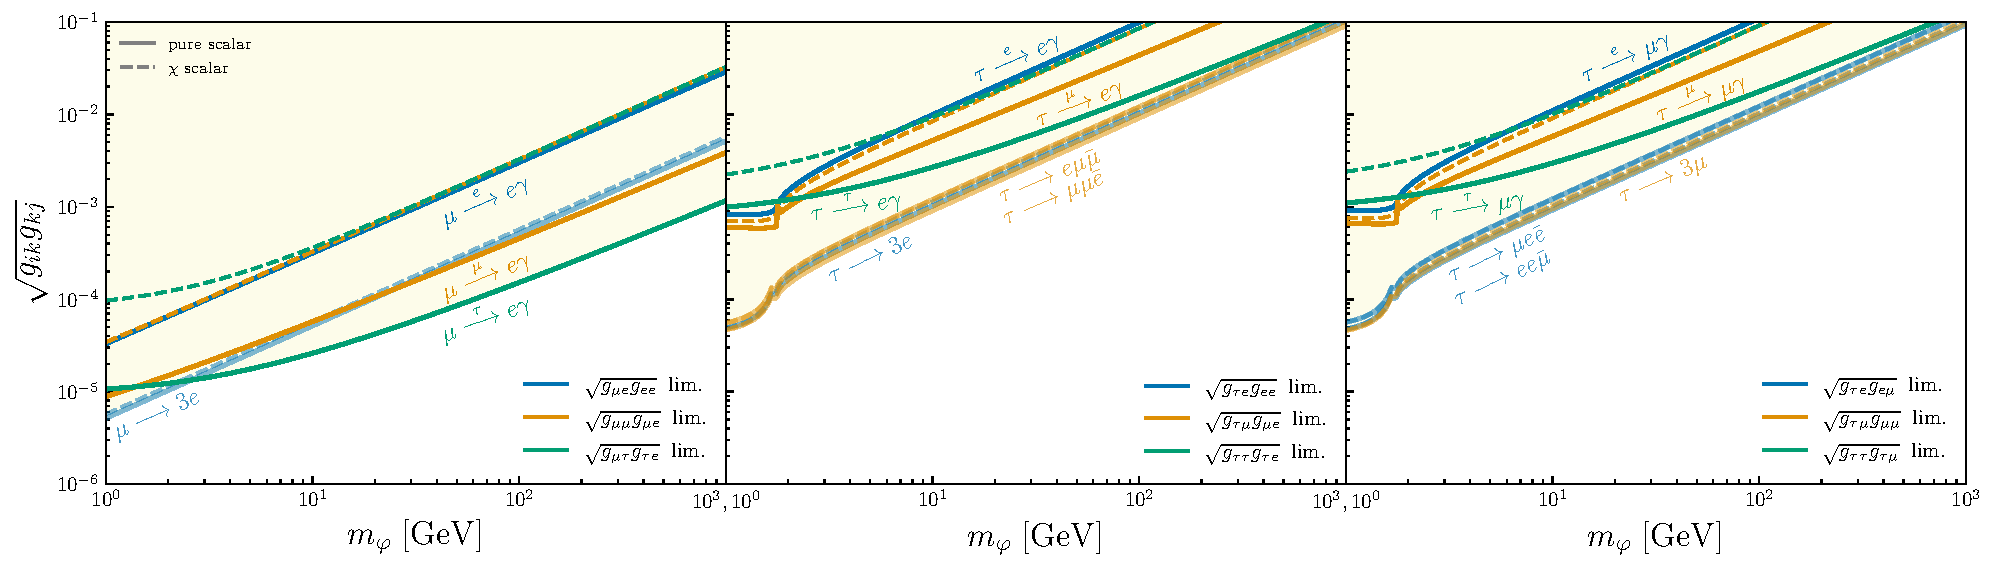
\includegraphics[width=\linewidth]{figures/chapter3/lfv_scalar_lepton_decay_limits.pdf}\\
 \makebox[0pt][l]{\hspace{-8.29cm}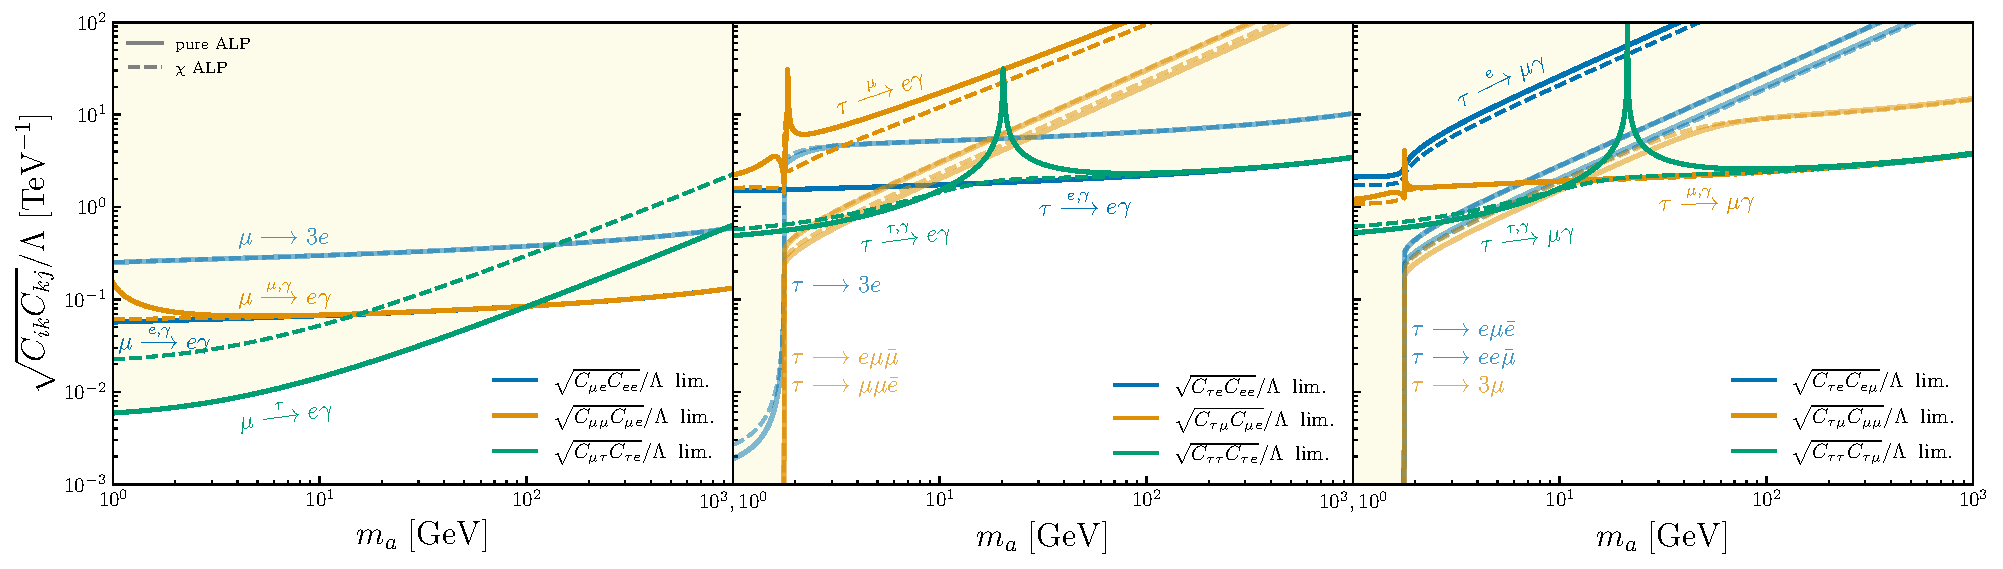
\includegraphics[width=\linewidth]{figures/chapter3/lfv_alp_lepton_decay_limits.pdf}}
    \caption[Constraints on LFV scalar and ALP couplings from LFV lepton decay limits.]{(Top) Limits (90\% CL) on the relevant LFV and LFC scalar couplings for the LFV decays $\ell_i \rightarrow \ell_j \gamma$ and $\ell_i\rightarrow\ell_j\ell_k\bar{\ell}_l$, assuming the interaction Lagrangian in Eq.~\ref{eq:LFV_scalar_int}. (Bottom) The same limits on the corresponding LFV and LFC ALP couplings in the interaction Lagrangian in Eq.~\ref{eq:LFV_ALP_int}, with $\Lambda = 10~{\rm TeV}$ (apart from the photonic contribution to the diagonal ALP vertex, the limits are unaffected by changes in $\Lambda$). The limits for pure (parity-conserving) particles are represented as solid lines, whereas the limits for chiral particles are dashed lines. }
    \label{fig:LFV_limits}
\end{figure}

The corresponding limits for LFV ALPs are shown in the bottom of Fig.~\ref{fig:LFV_limits}. For those limits on the product $\sqrt{C_{ii}C_{ij}}/\Lambda$, the photonic contribution is also included. As opposed to the complex scalar, most of the contributions to the ALP decay modes are largely independent of the chiral nature of the ALP, with the only exception being the $\mu \overset{\tau}{\longrightarrow} e\gamma$ decay mode. That said, this is by far (all couplings equal) the most dominant contribution to the $\mu\rightarrow e\gamma$ decay rate, due in part to the mass-dependence of the ALP coupling. Hence, this effect can be important in limits on LFV ALPs from the $\mu\rightarrow e\gamma$ decay. While the effect is not as drastic, we still see a factor of $\sim 4$ difference in the limits in Fig.~\ref{fig:LFV_limits}, corresponding to a factor of $\sim 250$ in the $\mu \rightarrow e\gamma$ decay rate.

Before ending this section, we reiterate that each of the limits presented in Fig.~\ref{fig:LFV_limits} is on a product of two couplings.  As a result, it is impossible to pin down constraints on any single flavor-violating (or flavor-conserving) coupling without fixing another. One can make some progress by appealing to naturalness or the minimal flavor-violating hypothesis \cite{Isidori:2012ts} in order to relate the size of the couplings, but this is not a fully general treatment. In particular, it is possible to construct symmetry-protected LFV interactions that completely evade the bounds in Figs.~\ref{fig:LFV_limits}. For a concrete  example, consider a $U(1)_{L_i - L_j}$ extension to the SM, along with a complex scalar field $\varphi$ of $L_i - L_j$ charge $+2$.  This particle has a singular non-zero coupling to the leptons, $g_{ij}$, and hence is not constrained at all by Fig.~\ref{fig:LFV_limits}.\footnote{This is partly due to the fact that the $\varphi$ preserves the flavor symmetry by carrying its own $e-\tau$ charge. In the event that the $U(1)_{L_e - L_\tau}$ symmetry is spontaneously broken, the resulting physical scalars of the theory will couple predominantly to $e\tau$, with only minor couplings to the other lepton currents.} Such a particle exists in the scalar spectrum in Ref.~\cite{Crivellin:2015mga} for $U(1)_{L_\mu - L_\tau}$. One can also consider particles with charge $+1$ under the $U(1)_{L_i - L_j}$, which have only two off-diagonal couplings and no diagonal-couplings, such as the $\phi$ in Ref.~\cite{Heeck:2011wj}. Something similar can also happen for an ALP which only couples to the lepton vector current instead of the axial-vector current (i.e. $C_L = C_R$ in Eq.~\ref{eq:ALP_int_from_UV}); then, the on-diagonal couplings are zero, which removes most of the constraints in Fig.~\ref{fig:LFV_limits}.

This leads us naturally into the next section: while singular couplings cannot be directly probed with the radiative and trilepton decay modes, they {\it can} be individually probed with the leptonic dipole moments (at least up to fine-tuned deconstructive interference between diagrams). For generic CP-violating couplings, the most stringent constraints come from the electron electric dipole moment. However, the contribution to the electric dipole moment from the models we consider vanish in the pure (pseudo)-scalar and chiral scenarios. These models can be probed complementarily by the lepton magnetic dipole moments, and can even be used to explain the electron and muon $g-2$ anomalies. 

\section{LFV Contributions to Lepton Electric and Magnetic Dipole Moments}\label{sec:edm_mdm}

The lepton electric and magnetic dipole moments are perhaps the most heavily scrutinized observables in modern particle physics. Whereas observables involving hadrons are rife with systematic error due to the non-perturbative nature of the strong interaction, leptons provide a clean environment which allows for very precise determination of their properties. 

\subsection{Electric Dipole Moments}\label{sec:edm}

While the electric dipole moment (EDM) of the electron has never been measured directly, it is constrained to a very high degree. The most stringent limit on the electron EDM comes from the University of Colorado, with $|d_e| < 4.1\times 10^{-30}~e\,{\rm cm}$ at the 90\% confidence level \cite{Roussy:2022cmp}. This is still some five orders of magnitude above the SM prediction of $|d_e|\approx 10^{-35}~e\,{\rm cm}$ \cite{Ema:2022yra},\footnote{Technically, the experimental bound in Ref.~\cite{Roussy:2022cmp} and the corresponding SM prediction \cite{Ema:2022yra} is of the quantity $d_e^{\rm equiv} = d_e^{\rm free} + r C_{S}$, where $d_e^{\rm free}\sim 6\times 10^{-40}~e\,{\rm cm}$ is the EDM of a free electron\cite{Yamaguchi:2020eub}, $C_S$ is the coefficient of an effective semileptonic electron-nucleon coupling, and $r$ is a constant which depends on the molecule used to compute the electric dipole moment, with $r \approx 1.5\times 10^{-20}~e\,{\rm cm}$ for a thorium monoxide molecule.} but can nonetheless provide strong bounds on new CP-violating physics in the charged lepton sector \cite{Cesarotti:2018huy,Pospelov:2005pr}. The muon and tau EDMs have also been indirectly constrained from their loop-level contributions to heavy atom EDMs, with $|d_\mu| < 1.9\times 10^{-20}~e\,{\rm cm}$ and $|d_\tau| < 1.6\times 10^{-18}~e\,{\rm cm}$ \cite{Ema:2021jds}. The corresponding SM predictions of $|d_\mu| = 10^{-42}e\,{\rm cm}$ \cite{Ema:2021jds} and $|d_\tau| \approx 3\times 10^{-37}~e\,{\rm cm}$ \cite{Mahanta:1996er}, far below the current experimental reach. While these constraints can also be used to limit CP-violating new physics, the resulting bounds are not very strong, so we will focus mainly on the electron EDM.

\subsection{Magnetic Dipole Moments}\label{sec:mdm}
The magnetic dipole moment (MDM) of the leptons (and in particular, the electron) have a special place in the history of quantum field theory. The MDM of a particle with charge $q$, mass $m$, and spin $S$ can generically be parametrized by $\mu = g\frac{q}{4m}S$, with non-relativistic quantum theory predicting $g = 2$ exactly for spin-1/2 particles. However, higher order corrections are expected from relativistic effects, which can be encoded in the {\it anomalous} magnetic moment, defined as the deviation of the $g$-factor from $2$, $a \equiv (g-2)/2$. In the 1940s, Tomonaga, Schwinger and Feynman independently used their theories of perturbative quantum electrodynamics at the time to calculate the electron anomalous magnetic moment $a_e$ to lowest order in the fine structure constant, each finding $a_e \approx \alpha/2\pi$~\cite{Tomonaga:1948zz,Schwinger:1948iu,Feynman:1948ur}. This was the first quantitative prediction of quantum electrodynamics, and it won Feynman, Schwinger, and Tomonaga the Nobel Prize in 1965 \cite{nobel1965physics}.

Now, the electron anomalous magnetic moment is the most precisely calculated and measured observable in physics. The theoretical prediction is so precise that its value is currently dependent on whether one uses the experimental value for the fine structure constant measured from Cesium (Cs)~\cite{Parker:2018vye} or Rubidium (Rb)~\cite{Morel:2020dww} atomic recoils, which deviate from each other at only one part per billion. If one uses the value of $\alpha({\rm Cs})$, the theoretical prediction is \cite{Parker:2018vye}
\begin{align}
    a_e^{\rm th.}({\rm Cs}) &= 1\,159\,652\,181.61(23)\times10^{-12},
\intertext{whereas for $\alpha({\rm Rb})$, \cite{Morel:2020dww} }
    a_e^{\rm th.}({\rm Rb}) &= 1\,159\,652\,180.252(95)\times10^{-12}.
\end{align}
Intriguingly, each of these is in modest disagreement with the current leading experimental value, in opposing directions. The leading experimental determination for $a_e$ is~\cite{Fan:2022eto}
\begin{align}
    a_e^{\rm exp.} &= 1\,159\,652\,180.59(13)\times 10^{-12}
\end{align}
corresponding to the anomalies
\begin{align}
    \Delta a_e(\rm Cs) = (-101 \pm 27)\times 10^{-14} , && \Delta a_e(\rm Rb) = (34 \pm 16)\times 10^{-14}.
\end{align}
In particular, there is a $-3.7\sigma$ anomaly in $\Delta a_e({\rm Cs})$ and a milder $+2.1\sigma$ anomaly in $\Delta a_e({\rm Rb})$.

While the muon anomalous magnetic moment is not measured as precisely as that of the electron, it has been the subject of immense scrutiny since the E821 Experiment at Brookhaven National Lab reported a $2.6\sigma$ deviation between their measurement of $a_\mu$ and the SM value at the time \cite{Muong-2:2001kxu}. This discrepancy has stood the test of time, through the completed analysis of E821 \cite{Muong-2:2006rrc} and the continuation of the experiment at Fermilab. As of 2021, the data analysis from Run 1 of the Fermilab $g-2$ experiment confirmed the Brookhaven result, finding a combined value of \cite{Muong-2:2021ojo}
\begin{align}
    a_\mu^{\rm exp.} &= 1165920.61(41)\times 10^{-9}
\intertext{Concurrently, the Muon $g-2$ Theory Initiative has reported an SM value of \cite{Aoyama:2020ynm} }
    a_\mu^{\rm th.} &= 1165918.10(43)\times 10^{-9}.
\end{align}
thus confirming the anomaly with
\begin{align}
    \Delta a_\mu &= 2.51(60)\times 10^{-9},
\end{align}
corresponding to a $4.2\sigma$ deviation.

The apparent anomalies in the muon and (to a lesser extent) electron anomalous magnetic moments are exciting indications of potential contributions from physics beyond the SM. However, it is important to temper our expectations. The disagreements for the electron $g-2$ anomaly are mild, and may disappear with more experimental data. While the muon anomaly is less likely to be a statistical fluke ($1$ in $10^5$), there is increasing evidence to suggest that the experimental result agrees with lattice calculations of the hadronic-vacuum-polarization (HVP) contribution to the muon $g-2$~\cite{Lehner:2020crt,Borsanyi:2020mff,Boccaletti:2024guq,Bazavov:2024eou}, indicating that the disagreement may lie within the data-driven approach used to determine the HVP. Recently, data analysis for Runs 2 and 3 of the Fermilab $g-2$ experiment was completed, confirming the experimental result with slightly more precision \cite{Venanzoni:2023mbe}, but they defer direct comparison with theory until the HVP discrepancy is resolved. Time will tell whether the tension between these experiments and the theoretical results remain; if they disappear, the electric and magnetic dipole moments can still be used to place constraints on new physics.

The lepton EDMs and MDMs are sensitive to any new physics involving leptons, the LFV scalars and ALPs in this chapter being no exception. These observables receive independent contributions from each non-zero coupling $g_{\ell\ell'}$, and hence can be used to probe individual couplings in isolation. To examine this effect, we begin by computing the contribution of LFV scalars and ALPs to the relevant dipole form-factors.


\subsection{Relevant Form Factors}\label{sec:diagonal_ff}
The most general gauge-invariant decomposition of the electromagnetic ($\ell_i \rightarrow\ell_i$ flavor-conserving) current into real, dimensionless form-factors is \cite{Nowakowski:2004cv}
\begin{align}
    \bar{u}_i(q_2)\Gamma_\mu^{i} u_i(q_1) &= e\bar{u}_i(q_2)\left[F_1^{i}(q^2)\gamma^\mu +  \frac{i\sigma^{\mu\nu}}{2m_i}q_\nu F_2^i(q^2) + \frac{\sigma^{\mu\nu}}{2m_i}q_\nu \gamma_5 F_3^i(q^2)\right.\nonumber\\ 
    &\left.\ \ \ \ \ \ + \frac{1}{2m_i}\left(q^\mu - \frac{q^2}{2m_i}\gamma^\mu\right)\gamma_5 F_4^i(q^2)\right]u_i(q_1).
\end{align}
Here, $F_1^i(q^2)$ is the electromagnetic charge, $F_2^i(q^2)$ is related to the magnetic dipole moment (MDM) form-factor, $F_3^i(q^2)$ is the electric dipole moment (EDM) form-factor, and $F_4^i(q^2)$ is the anapole form-factor. In particular, we have the freedom to define $F_1^i(0) = 1$ so that the electromagnetic charge is $e$. The benefit of decomposing the electromagnetic current in this form is that each of the form-factors $F^i$ is real-valued.\footnote{For $m_\varphi + m_j < m_i$, the form-factors have an imaginary part which reflects the fact that the particle $m_\varphi$ and the internal fermion $\ell_j$ can go on-mass-shell. These imaginary parts do not contribute to the dipole moments, but instead encode the probability that the parent lepton may decay via $\ell_i \rightarrow \ell_j \varphi$.} The MDM form-factor is related to the MDM via
\begin{align}
    \mu_i &\equiv g_i\frac{e}{4m_i} = \frac{e}{2m_i}\left(1 + F_2^i(0)\right).
\end{align}
The anomalous magnetic moment is then defined as $a_i \equiv (g_i - 2)/2 = F_2^i(0)$. The EDM form-factor is related to the EDM via
\begin{align}
    d_i & = -\frac{e}{2m_i}F_3^i(0).
\end{align}
With this in mind, we can compute the dipole moment form-factors for an LFV scalar and ALP with interactions governed by Eqs.~\ref{eq:LFV_scalar_int} and \ref{eq:LFV_ALP_int}. This surmounts to calculating the amplitude for the Feynman diagram on the left of Fig.~\ref{fig:LFV_vertex}. Using a similar decomposition as in Eqs.~\ref{eq:f_plus_minus}, we find using PackageX in Mathematica~\cite{Patel:2016fam} that the contribution to the dipole form factors are given by
\begin{align}
    F_2^{ij}(0) &= \frac{g_{ij}^2}{32\pi^2}\left[g_+(\mu_i, \mu_j)+g_-(\mu_i, \mu_j)\cos{2\theta_{ij}}\right]\label{eq:MDM_FF}\\
\intertext{and}
    F_3^{ij}(0) &= -\frac{g_{ij}^2}{32\pi^2}g_-(\mu_i, \mu_j)\sin{2\theta_{ij}}\cos{\delta_{ij}}\label{eq:EDM_FF}.
\end{align}
The functions $g_{\pm}$ are given by
\begin{align}
    g_+(x, y) &= \frac{2y}{x^2}\left[1+\frac{1 + x^2 - y^2}{x^2}\log{y} + \frac{(1+x^2-y^2)^2 - 2x^2}{\sqrt{(1 + x^2 - y^2)^2 - 4x^2}}{\rm arccosh}\left(\frac{1-x^2+y^2}{2y}\right) \right]
\intertext{and}
    g_-(x, y) &= -\frac{1}{x^3}\left[2+x^2  - 2y^2+\frac{2(1-y^2)^2 - 2x^2 y^2}{x^2}\log{y}\right.\nonumber\\
    &\ \ \ \ \ \ \ \ \left. - \frac{2[x^4 - (1-y^2)((1+x^2-y^2)^2-3x^2)]}{\sqrt{(1 + x^2 - y^2)^2 - 4x^2 }}{\rm arccosh}\left(\frac{1-x^2+y^2}{2y}\right)\right].
\end{align}
These can be computed directly from the transition dipole form-factors in  Eqs.~\ref{eq:F2ijk}-\ref{eq:F3ijk} by performing the limit $m_j \rightarrow m_i$ and replacing $m_k$ with $m_j$. In particular, we can identify
\begin{align}
    g_+(x, y) &= \lim_{z \rightarrow x}f_+(x, z, y)\\
    g_-(x, y) &= \lim_{z \rightarrow x}f_-(x, z, y).
\end{align}
While this identification is clear for the functional form of $F_2^{ij}(0)$, it is less apparent why $F_3^{ij}(0)$ should depend on only $g_-(x, y)$. Based on the form of Eq.~\ref{eq:F3ijk}, one would expect the functions $g_+'$ and $g_-'$ to appear in $F_3^{ij}$, where
\begin{align}
    g_+'(x, y) &= \lim_{z \rightarrow x}\frac{x+z}{x-z}f_+(x, -z, y)\\
    g_-'(x, y) &= \lim_{z \rightarrow x}\frac{x+z}{x-z}f_-(x, -z, y).
\end{align}
Explicit evaluation of the limits reveals $g_+'(x, y) = 0$ and $g_-'(x, y) = g_-(x, y)$, confirming Eq.~\ref{eq:EDM_FF}. 

Similar to the transition dipole form-factors, one can expect substantial differences between the contributions of chiral and pure scalars to $F_2^{ij}(0)$ when $|g_+(\mu_i, \mu_j)| \ll |g_-(\mu_i, \mu_j)|$, and at least marginal differences when $|g_+(\mu_i, \mu_j)| \sim |g_-(\mu_i, \mu_j)|$. The EDM form-factor $F_3^{ij}(0)$, on the other hand, is zero for pure and chiral scalars and ALPs, and more generally whenever $\delta_{ij} = \pi/2$ (regardless of $\theta_{ij}$).

When considering ALPs, we can use  Eqs.~\ref{eq:scalar_to_ALP} to re-express the form-factors in terms of the ALP parameters. We have 
\begin{align}
    F_2^{ij}(0) = \frac{C_{ij}^2}{32\pi^2 \Lambda^2}&\left[(m_i^2 + m_j^2 + 2m_i m_j\cos{2\Theta}_{ij})g_+(\mu_i, \mu_j)\right.\nonumber\\
    \ -&\left.\left(2m_i m_j + (m_i^2+m_j^2)\cos{2\Theta_{ij}} \right)g_-(\mu_i,\mu_j)\right]\\
    F_3^{ij}(0) = \frac{C_{ij}^2}{32\pi^2 \Lambda^2}&\left(m_i^2 - m_j^2\right)g_-(\mu_i, \mu_j)\sin{2\Theta_{ij}}\sin{\Delta_{ij}}.
\end{align}
There is an additional contribution to the magnetic dipole form-factor in the case of an ALP from the chiral anomaly. This contribution is \cite{Cornella:2019uxs}
\begin{equation}
    F_2^{i\gamma}(0) = -\frac{\alpha A_{ii}\sum_\ell A_{\ell\ell}}{2\pi^3}\frac{m_i^2}{\Lambda^2}\left[\log\frac{\Lambda^2}{m_i^2} - 1-\frac{x_i^2}{6}\log{x_i}+\frac{x_i}{3}+\frac{x_i+2}{3}\sqrt{x_i^2 - 4x_i}{\rm arccosh}\frac{\sqrt{x_i}}{2}\right].
\end{equation}
There is no additional contribution to the electric dipole form-factor.
\subsection{Approximations}\label{sec:diagonal_approx}
Like in the flavor-changing current case, we can examine various limits of the form-factor functions $g_{\pm}$. We will examine each of the cases $m_i \ll m_j$, $m_i = m_j$, and $m_i \gg m_j$.
\begin{enumerate}
    \item $i = j$\\
        This scenario is relevant for all the lepton dipole moments, given that the LFV particle has a flavor-conserving interaction. Unlike the $i = k > j$ case in the previous section, these results are exact, as there is no lepton mass ratio to expand around.
        \begin{align}
        g_+(\mu_i, \mu_j) &= 2-4x_i + 2x_i(x_i - 2)\log{x_i}- 4(x_i^2 - 4x_i + 2)\sqrt{\frac{x_i}{x_i - 4}}\log{\left(\frac{x_i + \sqrt{x_i(x_i - 4)}}{2\sqrt{x_i}}\right)}\nonumber\\
        g_-(\mu_i, \mu_j)&= 4-2x_i\log{x_i} + 4(x_i - 2)\sqrt{\frac{x_i}{x_i - 4}}\log{\left(\frac{x_i + \sqrt{x_i(x_i - 4)}}{2\sqrt{x_i}}\right)}
        \end{align}
        For ALPs, it is necessarily the case that $\theta_{ii} = \pi/2$, so only the function $g_-(\mu_i,\mu_j)$ contributes. Hence, there should not be any difference between a pure ALP or chiral ALP. However, there can be significant differences between the pure and chiral scalar contributions to the $i = j$ MDM form-factor.
    \item $i < j$\\
        This scenario is relevant for the electron dipole moments with an internal $\mu$ or $\tau$, and the muon dipole moments with an internal $\tau$. We have
        \begin{align}
        g_+(\mu_i, \mu_j) &= \frac{2\mu_i^2}{\mu_j^2}\left[\frac{2x_j^2 + 5x_j - 1}{3(x_j-1)^3}-\frac{2x_j^2}{(x_j-1)^4}\log{x_j}\right]\nonumber\\
        g_-(\mu_i,\mu_j) &= \frac{2\mu_i}{\mu_j}\left[\frac{1 - 3x_j}{(x_j-1)^2}+\frac{2x_j^2}{(x_j-1)^3}\log{x_j}\right].
        \end{align}
    Since $\mu_i \ll \mu_j$, the term involving $g_+$ is often neglected, but this can not be done for particles with a chiral interaction. Hence, we can expect significant differences between the contribution from pure and chiral scalars {\it and} ALPs.
    \item $i > j$\\
        This scenario is relevant for the muon dipole moment contributions with an internal $e$, and the tau dipole moments with an internal $\mu$ or $e$. We have
        \begin{align}
        g_+(\mu_i,\mu_j) &= -2 - 4x_i + 4x_i^2\log\frac{x_i}{x_i - 1}\nonumber\\
        g_-(\mu_i,\mu_j) &= \frac{4\mu_j}{\mu_i}\left[1 - \frac{x_i^2+1}{x_i - 1}\log\left(\frac{x_i}{x_i - 1}\right) + \frac{1}{x_i - 1}\log{x_j}\right].
        \end{align}
        Since $\mu_j \ll \mu_i$, the second term is typically neglected. As opposed to case (2), this is a valid approximation for all PV angles $\theta_{ij}$, so we shouldn't expect any major differences between the pure and chiral scenarios. 
\end{enumerate}

\begin{figure}[t!]
    \centering
    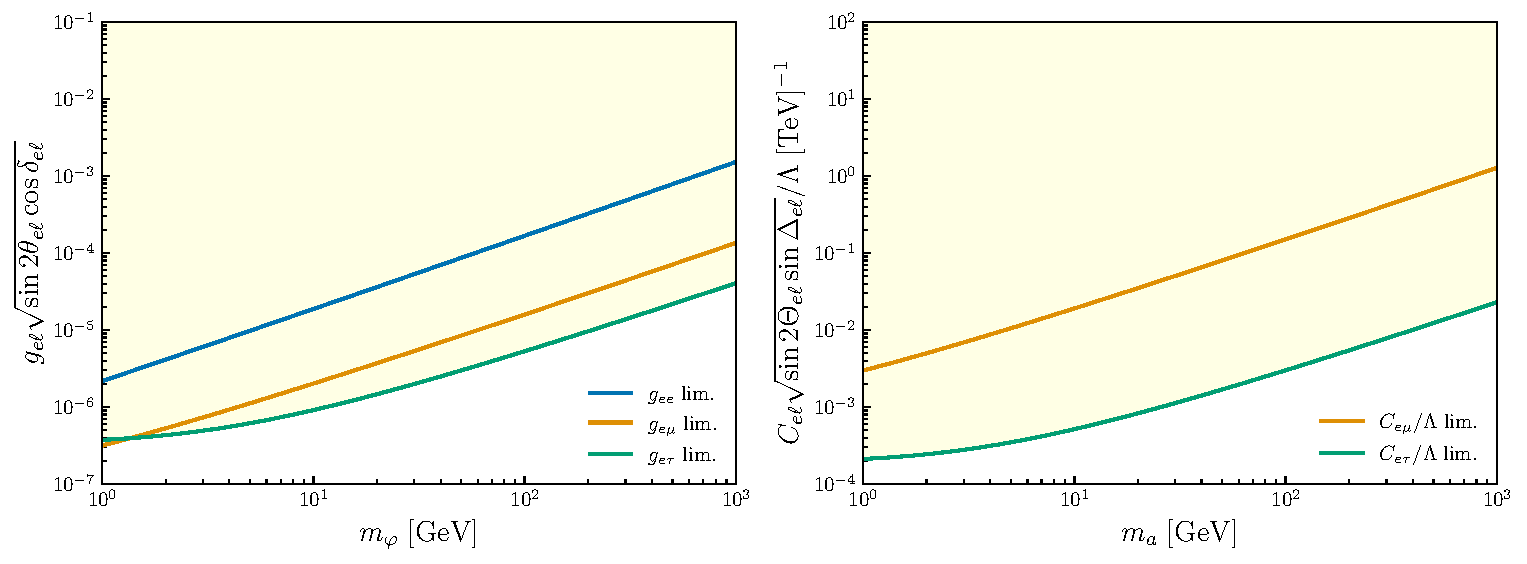
\includegraphics[width=\linewidth]{figures/chapter3/LFV_EDM_limits.pdf}
    \caption[Constraints on LFV scalar and ALP couplings from the lepton electric dipole moments.]{Limits on leptonic couplings for scalar (left) and ALP (right) from experimental constraints on the electron EDM. For the ALP, only the off-diagonal couplings are probed. For both pure and chiral particles, the bounds derived from the electron EDM vanish.}
    \label{fig:EDM_limits}
\end{figure}


\subsection{Electric dipole moment constraints}\label{sec:edm_limits}

Limits on LFV scalars from the electron EDM constraint are shown in Fig.~\ref{fig:EDM_limits}. Notably, these bounds far exceed the bounds obtained in Fig.~\ref{fig:LFV_limits}, and are able to constrain a singular coupling $g_{e\ell}$ rather than a product. However, they are only present when there is a significant amount of CP violation in the interaction (when $\sin{2\theta_{e\ell}}\cos{\delta_{e\ell}} \sim {\cal O}(1)$), and hence do not apply to pure {\it or} chirally-coupled particles. Similar bounds can be found for the $\mu$ and $\tau$ EDMs, but these are much less constrained by experiment, so the bounds are not competitive. 

\subsection{Magnetic dipole moment constraints}\label{sec:mdm_constraints}
For decades, the muon $g-2$ anomaly has captured the minds of particle physicists as a tantalizing hint at new physics, and more recently, the ($\alpha$-dependent) electron $g-2$ anomalies have also garnered considerable interest. However, recent studies indicate that the muon $g-2$ experiment may agree more closely with the theoretical result when using a lattice determination of the HVP~\cite{Lehner:2020crt,Borsanyi:2020mff,Boccaletti:2024guq,Bazavov:2024eou}, and the electron anomalies could very well be statistical flukes. In this section we will consider the less exciting scenario that these anomalies are resolved, or at the very least, that the new physics under consideration does not contribute to $a_e$ or $a_\mu$ at experimental levels. We will defer potential explanations of the $e$ and $\mu$ anomalies, in the event that they persist, to next section.



\begin{figure}[t!]
    \centering
    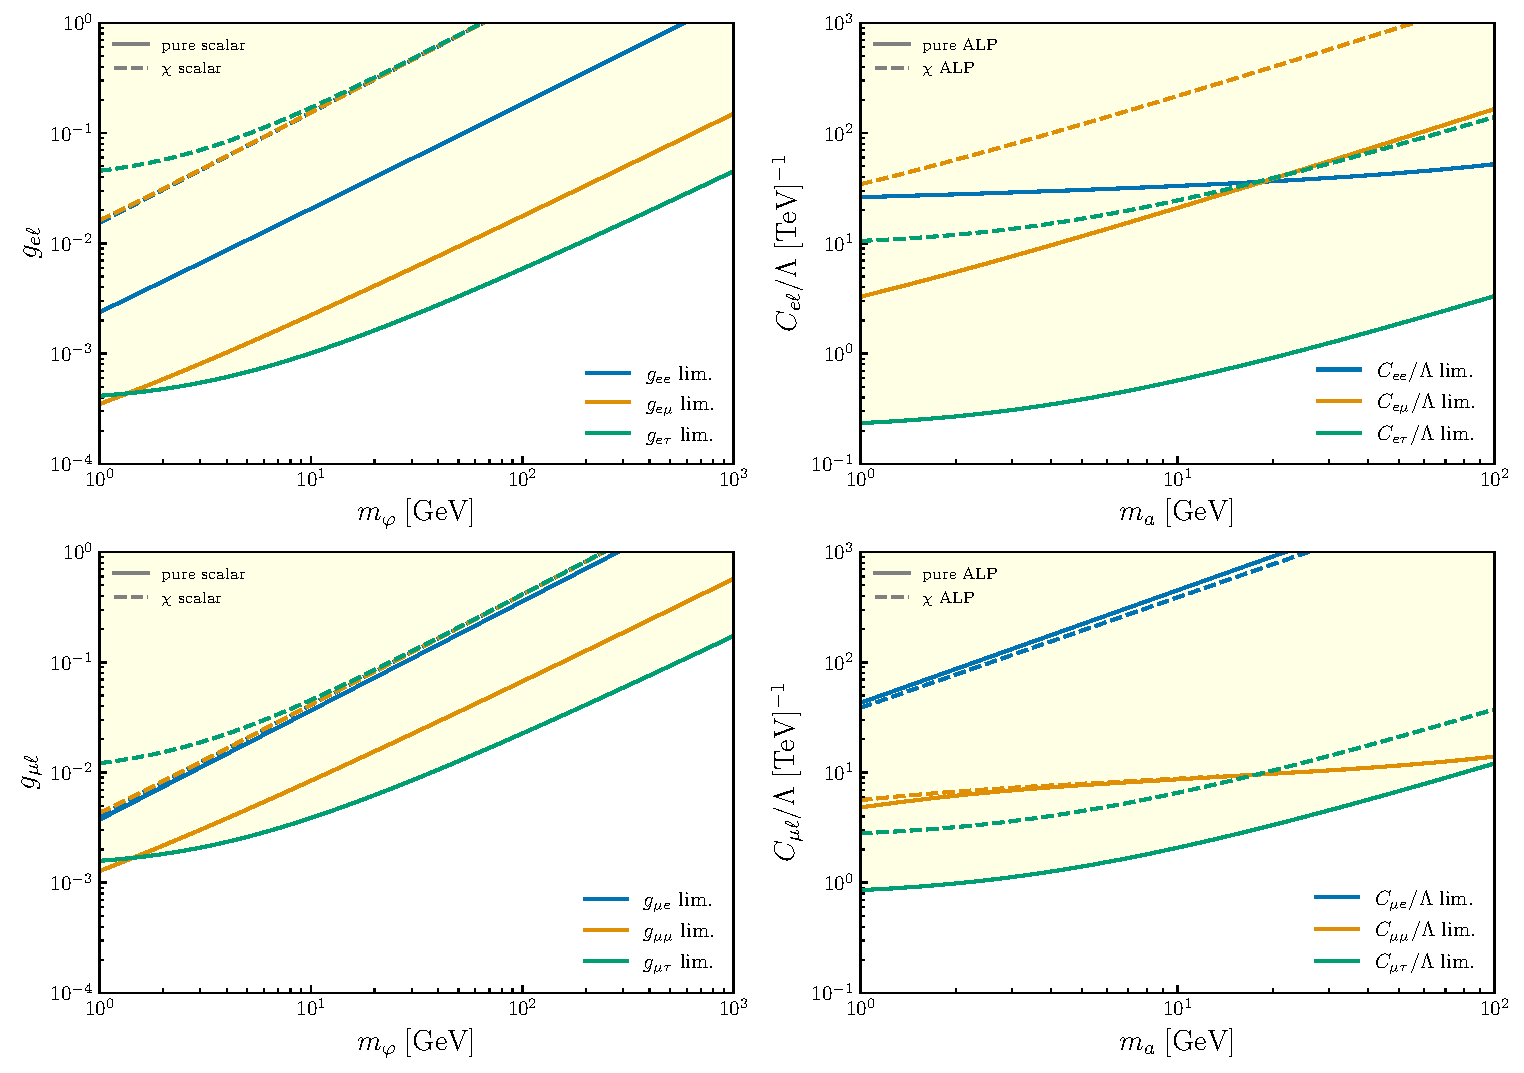
\includegraphics[width=\linewidth]{figures/chapter3/LFV_MDM_limits.pdf}
    \caption[Constraints on LFV scalar and ALP couplings from the lepton magnetic moments.]{Limits on scalar (left) and ALP ($\Lambda = 10~{\rm TeV}$, right) contributions to the anomalous magnetic moment of the electron (top) and muon (bottom), assuming the contributions lie within two standard deviations of the current experimental results. Pure scalars and ALPs are represented as solid lines, and chiral scalars and ALPs are represented as dashed lines. The limits are generated assuming $g_{\ell\ell'}$ is the only coupling present.}
    \label{fig:mdm_limits}
\end{figure}

To produce the limits, we assume an upper limit on the new physics contribution to the anomalous magnetic moment is $|\Delta a_\ell| < 2\sigma_\ell^{\rm exp}$, where $\sigma_{\ell}^{\rm exp}$ is the error in the experimental determination of $a_\ell$. For the electron $g-2$, we take the experimental error to be $\sigma_e^{\rm exp.} = 13\times 10^{-14}$ \cite{Fan:2022eto}. For the muon $g-2$, we use the combined experimental error from the Brookhaven results and Run 1 of the Fermilab results, $\sigma_\mu^{\rm exp} = 40\times 10^{-11}$ \cite{Muong-2:2021ojo}. We compute limits on a single coupling $g_{e\ell}$ (from $\Delta a_e$) or $g_{\mu\ell}$ (from $\Delta a_{\mu}$) under the assumption that all other couplings are zero. We compute contributions from both scalars and ALPs, and compare the pure and chiral scenarios. The results are shown in Fig.~\ref{fig:mdm_limits}, with pure scalar and ALP limits represented with solid lines and chiral scalar and ALP limits represented with dashed lines. 

Once again, we see a pronounced decrease in the contributions to the dipole moments for chiral scalars when compared to pure scalars. The largest of these differences is in the contribution of the scalars to $\Delta a_{e\tau}$, with a two order of magnitude suppression in the bound for $g_{e\tau}$. There are also substantial differences between chiral and pure scalars for the $g_{\mu \tau}$ bound, and the $g_{e\mu}$ bound from $\Delta a_{e}$ (but not $\Delta a_\mu$), which is in line with the notion that for the $i < j$ scenario (case (2)), there is an anticipated $m_i/m_j$ suppression in the form-factor for chiral particles.

We also see that more of the ALP channels are sensitive to a difference between pure and chiral couplings than for the LFV lepton decay limits obtained in Fig.~\ref{fig:LFV_limits} (for which only the $\mu \stackrel{\tau}{\longrightarrow}e\gamma$ mode was affected). In particular, the $\Delta a_{e\tau}$ channel is the most affected, with the bound on $C_{e\tau}$ decreasing by a factor of $\sim 50$ for chiral ALPs. The bounds on $C_{e\mu}$ from $a_e$ and $C_{\mu\tau}$ are also suppressed for chiral ALPs, albeit to a lesser degree. The on-diagonal contributions $\Delta a_{\ell\ell}$ are unaffected, which is in line with our expectation for ALPs, since (as mentioned previously) any ALP coupling to the vector current is illusory.

These bounds are considerably weaker than those obtained through radiative decays in Fig.~\ref{fig:LFV_limits}, but they allow us to isolate a single coupling (ignoring interference with other diagrams of a similar magnitude). They also indicate that the interactions of chiral particles are often less constrained than their parity-conserving counterparts, especially for LFV couplings. Concretely, we can consider the limit on $g_{\tau e}$ in Fig.~\ref{fig:mdm_limits} in conjunction with the limit on $\sqrt{g_{\tau e}g_{ee}}$ from Fig.~\ref{fig:LFV_limits} for $m_\varphi = 10~{\rm GeV}$. For pure scalars, $g_{\tau e} \lesssim 10^{-3}$ from Fig.~\ref{fig:mdm_limits} and $\sqrt{g_{ee}g_{\tau e}} \lesssim 10^{-3}$ from Fig.~\ref{fig:LFV_limits}, so we can parametrize the combined constraints as $g_{\tau e} \lesssim 10^{-3}\epsilon$ and $g_{ee} \lesssim 10^{-3}/\epsilon$ with $\epsilon < 1$. In contrast, the limits for chiral scalars entail $g_{\tau e}\lesssim 10^{-1}\epsilon$ and $g_{ee}\lesssim 10^{-5}/\epsilon$ for $\epsilon < 1$, allowing for a considerably larger off-diagonal chiral coupling $g_{\tau e}$. While this scenario may seem exotic, a VEV-less Higgs doublet $\varphi$ with charge $+2$ under $U(1)_{L_e - L_\tau}$ would have this property; such a particle is very unconstrained in spite of its strongly LFV coupling. More generally, any particle with a single off-diagonal coupling $g_{ij}\varphi \bar{\ell}_i[\cos{\theta_{ij}}+\gamma_5 \sin{\theta_{ij}}]\ell_j$ is perturbatively protected by a ${\Bbb Z}_4$ symmetry with, e.g., $Q(\varphi) = -1$, $Q(\ell_i) = i$ and $Q(\ell_j) = -i$. Such particles, if perverse, represent a region of the LFV scalar parameter space that is largely unconstrained by current experiments, especially when the interaction is chiral. In the next section, we will consider such particles in the context of the electron and muon $g-2$ anomalies.

\subsection{Explanations to electron and muon $g-2$ anomalies}\label{sec:g-2_explanation}
Here, we indulge in the possibility that the electron and muon $g-2$ anomalies are genuine, and new physics is needed to explain them. We focus on particles with a single non-zero leptonic coupling, $g_{\ell\tau}$, with $\ell = e~(\mu)$ for the electron (muon) anomaly. We will also assume that $\phi_{\tau\ell},\Phi_{\tau\ell} = 0$ and $\delta_{\tau\ell},\Delta_{\tau\ell} = \pi/2$, so as to evade the EDM constraints. Then, the interactions we consider are
\begin{align}
    {\cal L}_{\varphi} = g_{\tau \ell}\varphi\bar{\tau}(\cos{\theta} + \gamma_5\sin{\theta})\ell + {\rm H.c.}, && {\cal L}_a = C_{\tau \ell}\frac{\partial_\mu a}{\Lambda}\bar{\tau}(\sin{\Theta} + \gamma_5\cos{\Theta})\ell + {\rm H.c.}
\end{align}
Given that $m_\tau \gg m_\ell$, we ignore the $\theta$/$\Theta$-dependence in the conversion between the ALP and scalar couplings, so the ALP has an effective scalar coupling $g_{\tau \ell}^a \approx C_{\tau \ell}m_\tau / \Lambda$. In this limit, the PV angles are related via 
\begin{align}
    \Theta \approx \frac{m_\tau + m_\ell}{m_\tau - m_\ell}\left(\frac{\pi}{2} - \theta\right) \approx \left(1 + \frac{2m_\ell}{m_\tau}\right)\left(\frac{\pi}{2} - \theta\right).
\end{align}
\begin{figure}[t!]
    \centering
    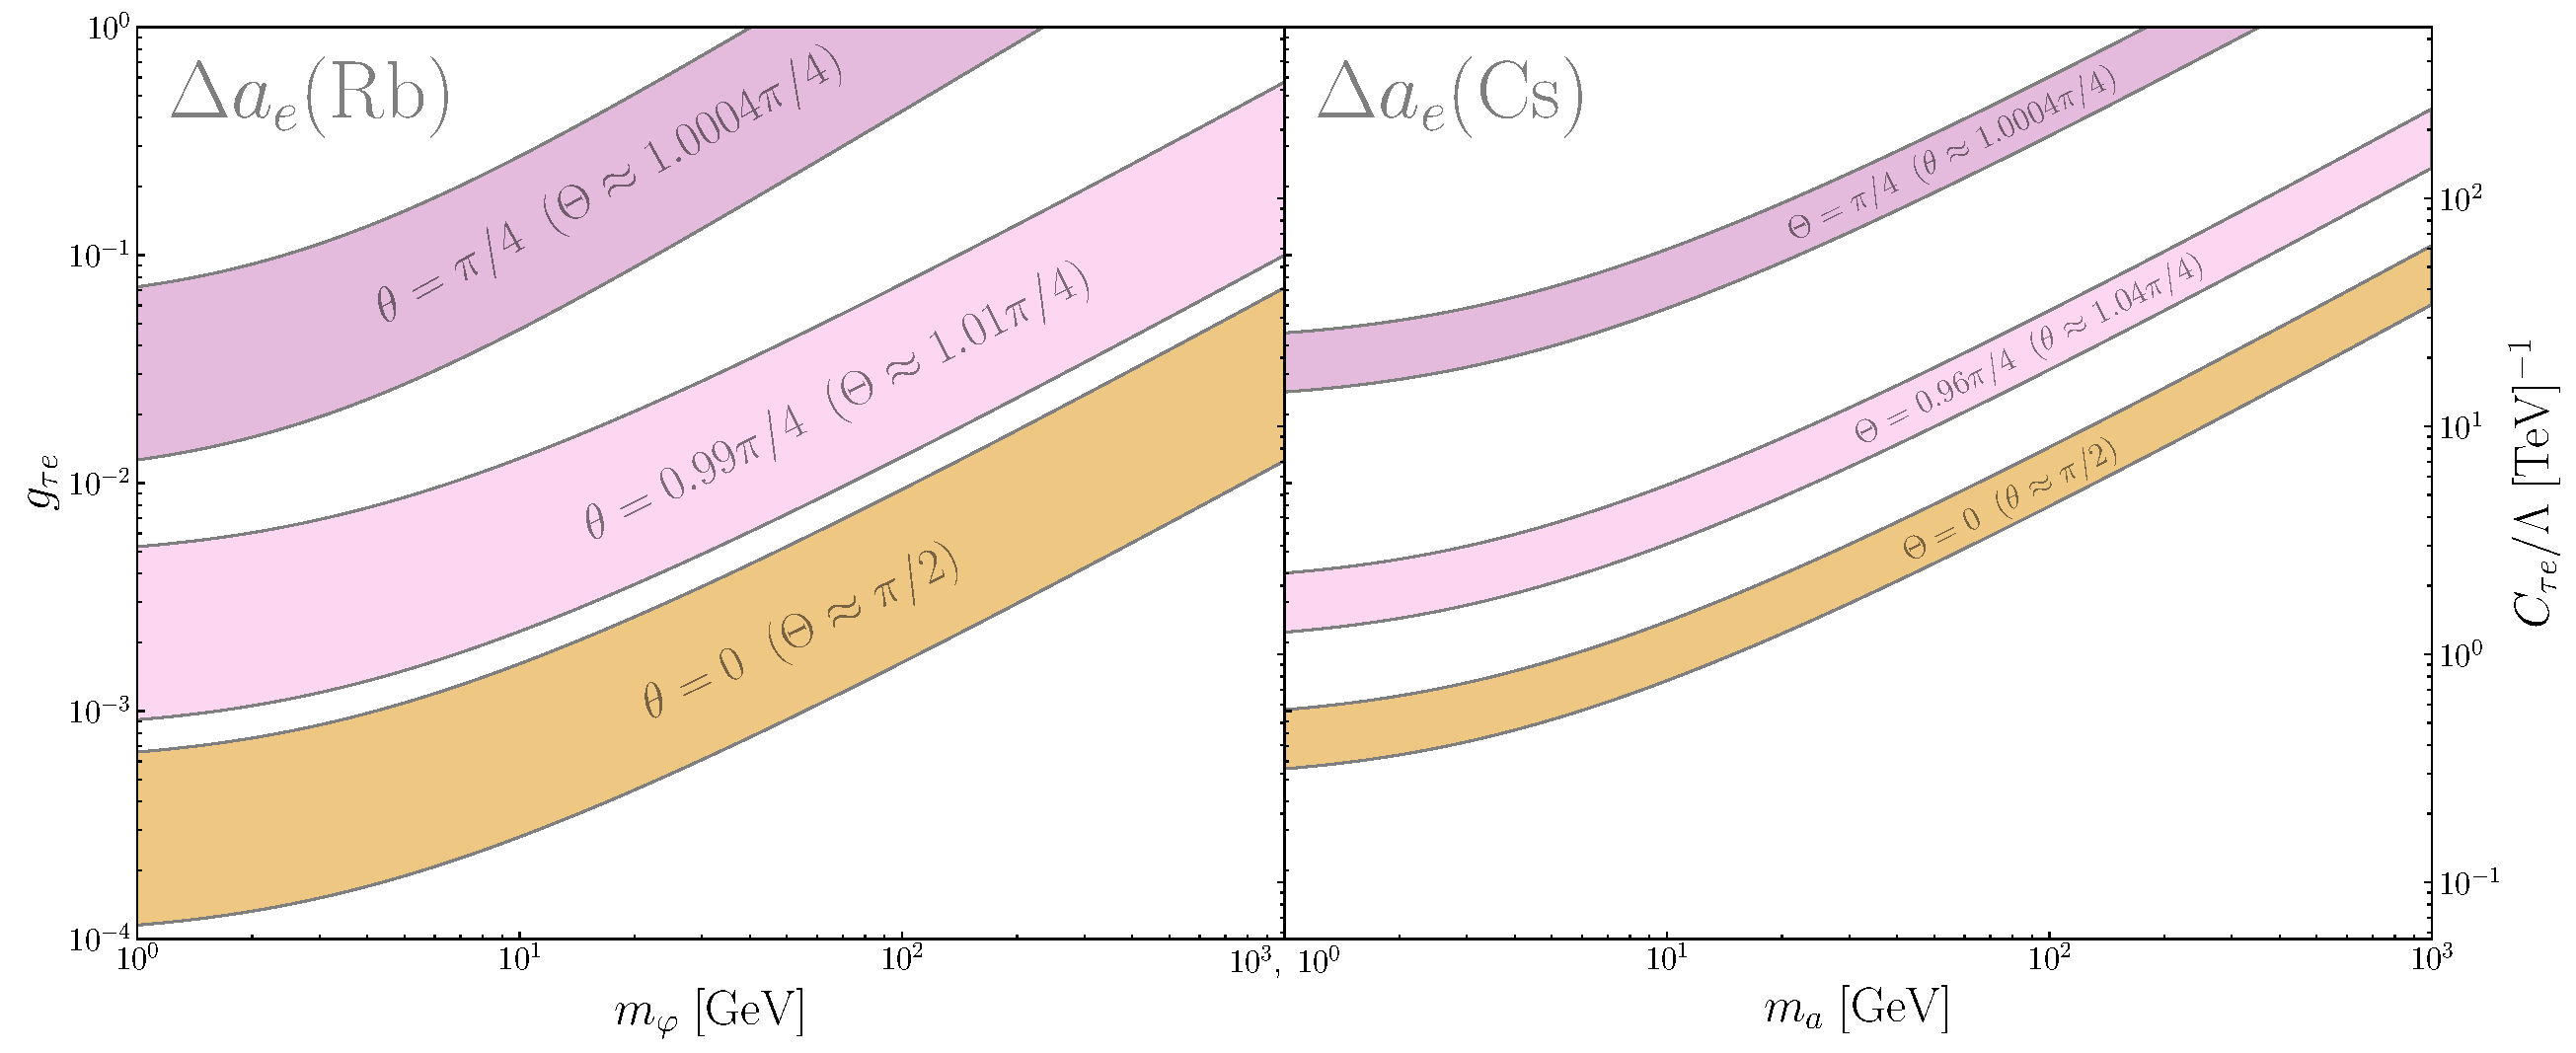
\includegraphics[width=\linewidth]{figures/chapter3/scalar_ALP_electron_g_2.pdf}
    \caption[LFV scalar and ALP explanations to electron $g-2$ anomalies.]{Viable explanations for both the Cesium and Rubidium electron $g-2$ anomalies at $2\sigma$ for a scalar (ALP) with flavor off-diagonal coupling $g_{\tau e}$ ($C_{\tau e}$) and PV angles $\theta$ ($\Theta$). We note that chiral ($\theta$, $\Theta = \pi/4$) solutions require much larger couplings, but this effect is very sensitive to even slight deviations in the angle.}
    \label{fig:electron_anomaly_explanations}
\end{figure}
To explore the full role of the PV angle, we consider explanations to each of the anomalies for three different PV angles: chiral ($\theta$ or $\Theta = \pi/4$), parity-conserving ($\theta$ or $\Theta = 0$), and a representative angle in between. We begin with explanations for the electron $g-2$ anomalies using $\alpha({\rm Rb})$ and $\alpha({\rm Cs})$ in Fig.~\ref{fig:electron_anomaly_explanations}, noting that $\Delta a_e({\rm Rb}) > 0$ while $\Delta a_e({\rm Cs}) < 0$. While we explore a variety of PV angles, it is well known that pure scalars contribute a {\it positive} contribution to the lepton dipole moments, whereas pure pseudoscalars contribute an {\it negative} contribution.\footnote{This is technically only valid for on-diagonal contributions and contributions with a heavier internal lepton. For contributions with a lighter internal lepton, both scalars and pseudoscalars (and anything in between) have a positive contribution.} To emphasize this point, we primarily consider a scalar explanation to the {\it positive} Rubidium anomaly for the pure and chiral scenarios $\theta = 0$ and $\theta = \pi/4$, as well as a near-chiral angle $\theta = 0.99\pi/4$, with the corresponding ALP PV angles $\Theta$ shown in parentheses. Similarly, we consider an ALP explanation to the {\it negative} Cesium anomaly, for pure and chiral scenarios $\Theta = 0$  and $\Theta = \pi/4$, as well as a near-chiral angle $\Theta = 0.96\pi/4$, with the corresponding scalar angles $\theta$ shown in parentheses. It is interesting to note just how delicate the chiral suppression is: for even a $1\%$ deviation in the PV angle, the $g_{\tau e}$ required to explain the anomalies approaches the parity-conserving explanation. Hence, if one is interested in this chiral effect, any higher-order non-chiral contributions must be suppressed by at least the ratio $m_e/m_\tau$.
\begin{figure}[t!]
    \centering
    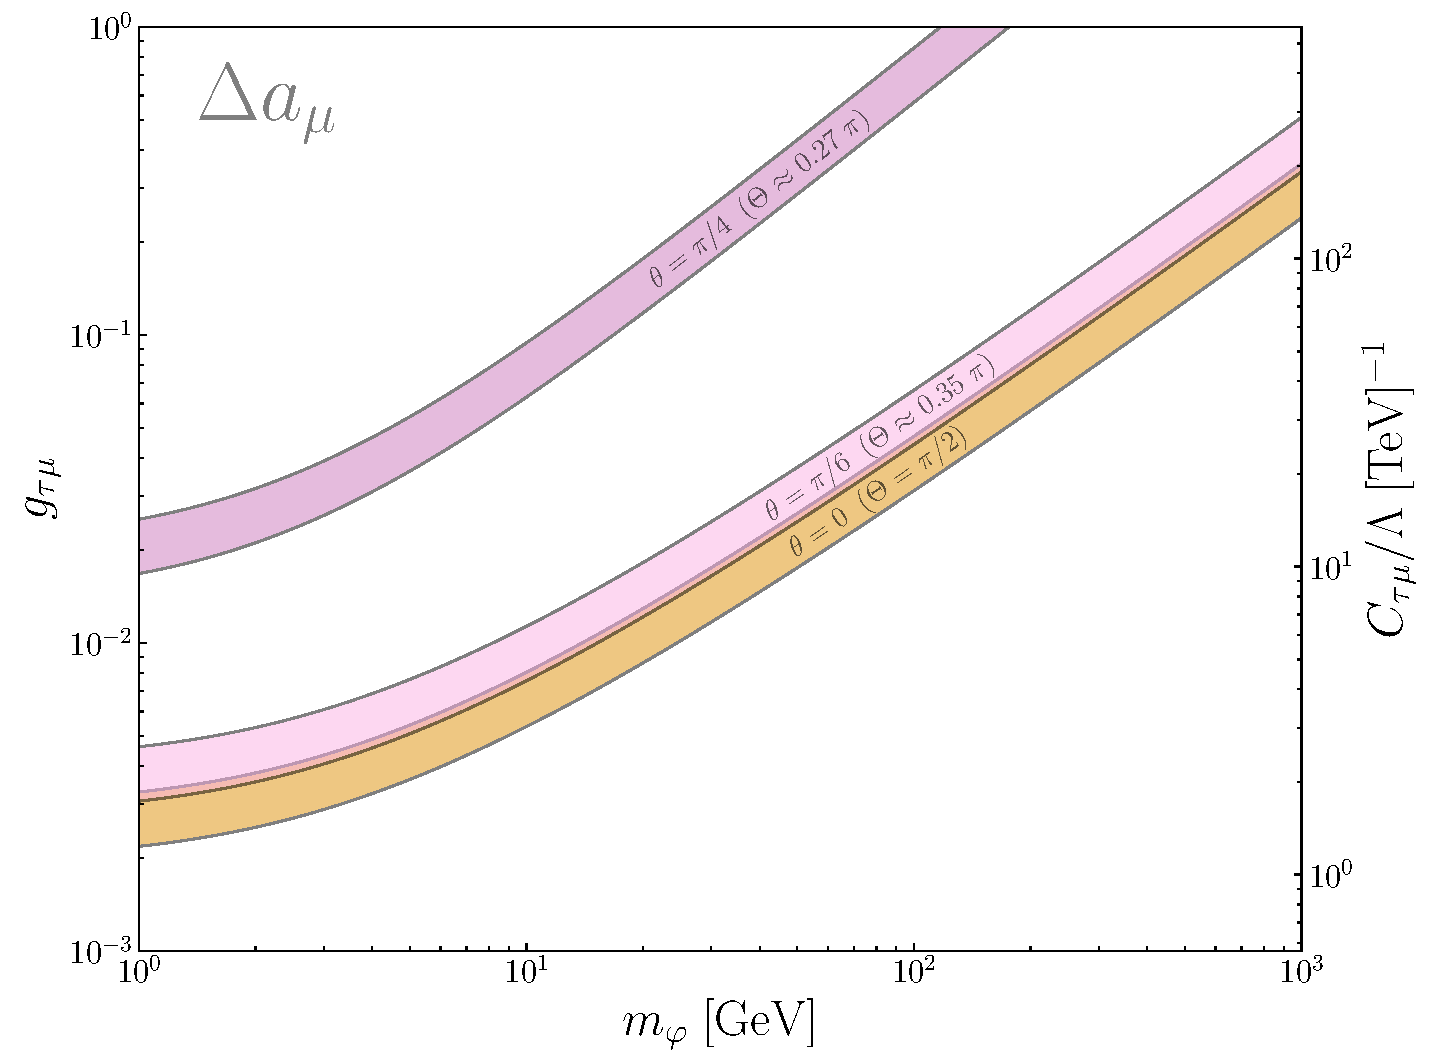
\includegraphics[clip,width=0.55\linewidth]{figures/chapter3/scalar_ALP_muon_g_2.pdf}
    \caption[LFV scalar and ALP explanations to muon $g-2$ anomaly.]{Viable explanations for the muon $g-2$ anomaly at $2\sigma$, for a scalar (ALP) with flavor off-diagonal coupling $g_{\tau\mu}$ ($C_{\tau\mu}$) and PV angles $\theta$ ($\Theta$). Like the scalar case, the chiral solutions require much larger couplings, but this effect is very sensitive to deviations in the PV angle.}
    \label{fig:muon_anomaly_explanation}
\end{figure}

We repeat this analysis for explanations to the muon $g-2$ anomaly in Fig.~\ref{fig:muon_anomaly_explanation}. Since $\Delta a_\mu > 0$, we primarily consider scalar explanations to the anomaly for the chiral scenarios $\theta = 0$ and $\theta = \pi/4$, as well as an intermediate angle $\theta = \pi/3$, with the corresponding ALP angles shown in parentheses. Once again, we see that the chiral suppression of the contribution to $a_\mu$ requires a much larger coupling, but this effect is very sensitive to deviations from $\theta = \pi/4$. 

For each of the anomalies, the couplings required for an explanation are quite large, especially for chirally-coupled particles. However, we note that these couplings in isolation are entirely unconstrained by modern experiments. In Chapter~\ref{upc}, we will explore the degree to which this range of couplings can be probed at lepton-ion colliders and beam-dump experiments for scalars, and in  Chapter~\ref{alp_collider} we will repeat this analysis for ALPs.
